\documentclass[11pt]{article}
\usepackage[a4paper,top=0.85in,bottom=0.85in,left=0.88in,right=0.88in]{geometry}
% ---- Times New Roman (text + math) ----
\usepackage{newtxtext}
\usepackage{newtxmath}
\usepackage[T1]{fontenc}
\usepackage[utf8]{inputenc}
\usepackage{graphicx}
\graphicspath{{figures/}{../figures/}{./}}
\usepackage{booktabs}
\usepackage{amsmath}
\usepackage{amssymb}
\usepackage{caption}
\usepackage{microtype}
% ---- clickable numeric citations + bookmarks ----
\usepackage[colorlinks=true,linkcolor=black,citecolor=blue,urlcolor=blue,linktoc=all]{hyperref}
\usepackage{url}
\usepackage{seqsplit}
\usepackage{float}
\usepackage[section]{placeins}
% ---- float placement: let a figure and its two tables group near their
%      in-text references instead of drifting to the bottom of a later page ----
\setcounter{topnumber}{3}
\setcounter{totalnumber}{4}
\setcounter{bottomnumber}{1}
\renewcommand{\topfraction}{0.92}
\renewcommand{\bottomfraction}{0.5}
\renewcommand{\textfraction}{0.08}
\renewcommand{\floatpagefraction}{0.8}
% ---- page-fit: modest spacing, discourage orphan/widow lines ----
\captionsetup{font=small,labelfont=bf,skip=4pt}
\clubpenalty=10000
\widowpenalty=10000

\setlength{\parskip}{0.15em}
\setlength{\parindent}{1.2em}
% ---- front-matter lists: keep the standard article/tocloft look (bold section
%      titles + bold page numbers, regular-weight subsections, dot leaders), with
%      only a modest before-skip tightening so ToC + LoF + LoT fit one page ----
\usepackage{tocloft}
\setlength{\cftbeforesecskip}{2pt}
\setlength{\cftbeforesubsecskip}{1pt}
\setlength{\cftbeforefigskip}{1pt}
\setlength{\cftbeforetabskip}{1pt}
\renewcommand{\cftsecfont}{\bfseries}
\renewcommand{\cftsecpagefont}{\bfseries}
\title{}\author{}\date{}
\begin{document}
% ---- Title and author block ----
\title{\vspace{-1.5em}One Capability or Many?\\ Testing the Economic Validity of Frontier AI Evaluation}
\author{Louis Yiven Zhu\\
\small Department of Statistics, London School of Economics and Political Science}
\date{}
\maketitle

\begin{abstract}
\noindent
Frontier-model leaderboards increasingly report ``economic'' benchmarks that aim to measure performance
on professionally valuable work, such as software engineering, banking workflows, and other job-like
tasks. Whether these benchmarks capture a distinct economic capability, or merely re-express the general
capability signal that all benchmarks share as models improve, is a question of construct validity that
has not been tested directly. We address it on a pinned snapshot of 421 frontier model configurations,
of which 96 carry the complete twelve-benchmark battery that the structural analysis requires, framing
benchmark validity as a latent-variable measurement problem. We combine exploratory factor analysis
under an oblique rotation with a leave-one-benchmark-out predictive test, so that structural and
predictive evidence are assessed against pre-registered thresholds. A single factor accounts for 74.5\%
of common variance and is strongly associated with model release date ($R^2=0.51$); residualising on
release date reduces that share to 59.6\%, a 14.9-point drop whose bootstrap interval straddles our
15-point discriminance threshold, so the effect is indistinguishable from the threshold at this sample
size. Our dimensionality rule retains a single factor, so the registered distinctiveness test is
reported as not supported. When we extract more factors than that rule selects,
the economic benchmarks do separate, and the separation carries out-of-sample weight, improving prediction
of held-out economic scores over a single general-capability index on three of the four economic
benchmarks (pooled $\Delta\mathrm{MSE}=0.037$, 95\% bootstrap interval $[0.019, 0.055]$). Economic
benchmarks therefore carry limited, incremental validity. They refine a dominant progress factor at the
margin while remaining largely explained by it. All hypotheses are pre-registered, the failing and
near-threshold tests are reported as such, and every input is hash-pinned for exact reproduction.
\end{abstract}

\vspace{0.5em}
\noindent\textbf{Keywords:} construct validity; benchmark evaluation; large language models; frontier AI;
psychometrics; exploratory factor analysis; latent-variable models; economic capability; predictive
validity; pre-registration; reproducibility.
\vspace{0.5em}

\newpage
{\setlength{\parskip}{0pt}
\tableofcontents
\vspace{0.6em}
\listoffigures
\vspace{0.6em}
\listoftables
}

\newpage
% ======================================================================
% Shared body content for both single- and two-column builds.
% All numbers are verbatim from the canonical result CSVs in data/processed/.
% ======================================================================

\section{Introduction}\label{sec:intro}

\subsection{Motivation and research questions}\label{sec:motivation}
Public leaderboards have become the dominant instrument through which frontier language models are
compared, procured, and governed, and a recent shift in what they report raises a measurement question
with direct economic stakes. Alongside academic knowledge tests such as GPQA and Humanity's Last Exam,
leaderboards now report \emph{economic} benchmarks such as GDPval, the $\tau$-Bench family, and
terminal or agentic coding suites, all designed to proxy paid professional work and multi-step tool use.
Whether these economic benchmarks deserve to be read as a separate column of the leaderboard depends
on what they actually measure. If they capture a capability distinct from general test-taking ability,
they carry information that a single ``intelligence'' score cannot, and reporting them separately is
warranted. If instead they largely re-express one dominant axis of model progress, then a separate
economic column overstates what the leaderboard knows. This is a question of construct validity, of
whether a measurement captures the theoretical construct it claims to, and recent work argues that
construct validity is systematically under-examined in AI evaluation \cite{bean2025,kearns2026}.

We make the question empirical and answer it with two machine-learning tasks under a pre-registered design. A snapshot of frontier models scored across twelve benchmarks is framed as a psychometric problem
in which benchmarks are items, models are respondents, and scores are the observed responses from which
latent capability structure is inferred. Two complementary research questions organise the analysis. The
first concerns structure. How many latent capabilities does the battery measure? Is a dominant axis
merely an artefact of release date and scale, and do the economic benchmarks occupy a separable position
once that axis is controlled? The second concerns prediction: does a multi-factor representation forecast
a model's held-out economic-benchmark score more accurately than a single general-ability index? The
first asks whether an economic factor exists in the correlational structure. The second asks whether, if
it exists, it carries information that survives out of sample.

\subsection{Related work}\label{sec:related}
Our study sits within a small but growing literature that treats LLM benchmarks as measurement
instruments open to measurement error. Bean et al.\ \cite{bean2025} review 445 benchmarks and
find that only a minority justify their construct validity or apply any statistical test, which
motivates precisely the kind of psychometric scrutiny we attempt here. Kearns \cite{kearns2026} makes that scrutiny quantitative. Fitting factor models to the Open LLM Leaderboard, Kearns shows that a dominant latent factor explains roughly 72\% of communal variance and correlates with model scale, while
partialling scale out redistributes that variance across several factors. That $72\%\rightarrow41\%$
correction is both the template for our residualisation and an external calibration
point for our own numbers, though Kearns studies academic suites and does not isolate
the economic column we target here. Our residualisation is designed to correct exactly the single-factor
reading that leaves release timing and scale uncontrolled, named in the registered plan as robustness item R4.

A second strand concerns how benchmark performance drifts over time. Akhtar, Reuel et al.\
\cite{akhtar2026} find that benchmark age and test-set scale are the strongest predictors of lost
discriminative power. Release date is therefore a first-order confound
when capabilities are compared across a moving frontier, and we residualise on
it before interpreting any factor structure. Reuel, Ghosh et al.\ \cite{reuel2026} map
coverage gaps across social-impact evaluations and argue that the dimensions a suite surfaces are
themselves a validity question. This supports our focus on whether economic capability is measured
separately or folded into a general score.

Methodologically, the contribution is the measurement design. It is built from established multivariate tools: exploratory factor analysis
with oblique rotation \cite{thurstone1947}, parallel analysis \cite{horn1965} and the scree criterion
\cite{cattell1966} for dimensionality, sampling-adequacy diagnostics \cite{kaiser1974,bartlett1950},
silhouette \cite{rousseeuw1987} and gap-statistic \cite{tibshirani2001gap} cluster validation,
regularised and tree-based regression \cite{hoerl1970,zou2005,breiman2001,friedman2001}, SHAP
attribution \cite{lundberg2017}, and the bootstrap \cite{efron1993}. The regression learners and
cross-validation use scikit-learn \cite{pedregosa2011}. The factor analysis uses the
\texttt{factor\_analyzer} package and SHAP its own reference implementation \cite{lundberg2017}.

\subsection{Contributions}\label{sec:contributions}
The paper makes four contributions, and each addresses a gap the existing literature leaves open. First,
it asks whether the \emph{economic}
column of a frontier leaderboard measures a capability distinct from general test-taking, where earlier
factor-analytic studies \cite{kearns2026} examined academic suites and treated capability as a single
undifferentiated construct. The economic benchmarks that now drive procurement and policy claims have
not previously been subjected to a construct-validity test, and that target is the paper's
central novelty. Second, it isolates model release date as a first-order confound and residualises on it
before reading any factor structure. What looks like one dominant
capability axis is then shown to be substantially a temporal artefact. Third, it introduces a leave-one-benchmark-out predictive-validity test that recasts the distinctiveness question as an out-of-sample forecast. This is a stronger and more decision-relevant criterion than in-sample loading patterns, since a benchmark
that adds nothing to prediction of held-out economic performance adds nothing a practitioner can use.
Fourth, it delivers the whole analysis under a pre-registered protocol with hash-pinned inputs, reporting
the near-threshold H2(ii) result and the not-supported H3 verdict alongside the confirmed ones
and documenting every deviation from the registered plan.

\subsection{Scope and non-goals}\label{sec:scope}
Fixing scope in advance keeps the claims disciplined and guards against over-reading a cross-sectional,
observational result. In scope is a construct-validity analysis of the economic benchmarks on a single
hash-pinned leaderboard snapshot, using exploratory factor analysis and clustering for structure and a
leave-one-benchmark-out regression for predictive validity, under four pre-registered hypotheses with
pre-specified thresholds. Several extensions are left to future work. The analysis is exploratory, and makes no confirmatory claim. It claims no validated measurement model on fresh data, and it uses aggregate
scores in place of item-level responses. It tests internal economic validity, the correlational and
predictive structure, and leaves external economic impact such as professional usage or revenue for later
work. Finally, it analyses one cross-section without saturation dynamics and treats published scores as
given, so it makes no causal claim. The residualisation identifies date as a strong correlate of the
general factor without establishing cause.

\section{Data}\label{sec:data}

\subsection{Source and provenance}\label{sec:source}
The primary data set is a snapshot of the Artificial Analysis model leaderboard \cite{aa2026}, captured
on 6 July 2026 directly from the public leaderboard page and pinned by its SHA-256 hash
(\texttt{6f19f8\ldots04de6}; the full manifest appears in Appendix~\ref{app:provenance}). The snapshot
contains 548 model configurations with per-benchmark scores, release dates, and provider metadata. A
secondary source, the Epoch AI Notable AI Models data set (CC-BY 4.0) \cite{epoch2026}, supplies
training-compute figures for a subset of models and is used only for a scale robustness check. Both
snapshots travel with the submission bundle, so every number in this paper is reproducible from fixed
inputs and neither source requires re-running a model.

\subsection{The benchmark battery}\label{sec:battery}
We analyse the twelve benchmarks that survive the coverage rule of Section~\ref{sec:inclusion}, grouped
into five capability blocks. Four are economic benchmarks in the sense of proxying paid professional or
agentic work, and the remainder span academic knowledge, scientific coding, long-context retrieval, and
instruction following. Appendix Table~\ref{tab:battery} describes each benchmark, the construct it targets, and
its coverage in the analysis snapshot.

\subsection{Inclusion rule and analysis grids}\label{sec:inclusion}
To avoid selecting benchmarks or models on the very outcomes under study, the coverage rule was fixed in
advance. A benchmark is retained if at least sixty models carry a score, and a model is retained if it
carries at least eight of the thirteen sufficiently-covered benchmarks. Thirteen of fourteen candidate
benchmarks pass. One agentic benchmark, APEX-Agents with twenty-six models, is dropped for sparsity, and
one multimodal benchmark, MMMU-Pro, is demoted to a sensitivity-only role. This leaves twelve primary
benchmarks and 421 model configurations. These 421 rows are configurations, since a single base
model can appear under several reasoning or effort settings. The registered analysis
deduplicates to one row per base model as robustness check R1 (Appendix~\ref{app:robust}), and we retain
the configuration level for the primary analysis as the more conservative choice.

Because the economic benchmarks are scored on far fewer models than the academic core, a single grid
cannot serve both analyses, so we work with two. The complete-case grid of 96 models scored on all
twelve benchmarks is the only grid on which the economic block is complete and carries all structure
hypotheses. The dense grid of 409 models scored on the nine near-universal benchmarks is used for model
clustering, where sample size matters more than economic completeness. This completeness-versus-sample
trade-off is the central data-design decision, and we flag it wherever it bears on a result.

\subsection{Preprocessing and encoding}\label{sec:preproc}
Three preprocessing decisions shape every downstream result. The benchmarks are reported on
incommensurable scales. Some are accuracy fractions, one is a hallucination-penalised score, and GDPval
is an Elo rating.\footnote{GDPval Elo ratings come from pairwise human preference comparisons on economically valuable tasks, so a higher rating means more often preferred, on a scale with no fixed maximum.} Each benchmark is therefore z-standardised before any analysis, using training-fold statistics only
in the supervised task. Standardisation keeps the variance
decomposition interpretable and stops the widest-range benchmark from dominating the covariance. GDPval
is treated as a continuous target on its own standardised
scale and excluded from the accuracy-only logit-transform check. The rung~(v) covariates
enter as one-hot indicators for reasoning capability and open-weights status,
log-parameters for parameter count, and a binary flag for undisclosed counts, so
missingness is modelled as information and never silently imputed.

\section{Exploratory data analysis}\label{sec:eda}
Exploratory analysis is conducted on the modelling data before any model is fitted. The marking guidance asks for it, and the choices it surfaces (which grid, whether to residualise,
how many factors to expect) should be informed by the data and never imposed on it. We examine
coverage and missingness, correlation structure, and temporal patterns, summarised in
Figure~\ref{fig:eda}. All standardisation and model fitting in later sections is performed on the
training portion of each split only, so the exploratory views here characterise the data without leaking
test information into the models.

\begin{figure}[htbp]
  \centering
  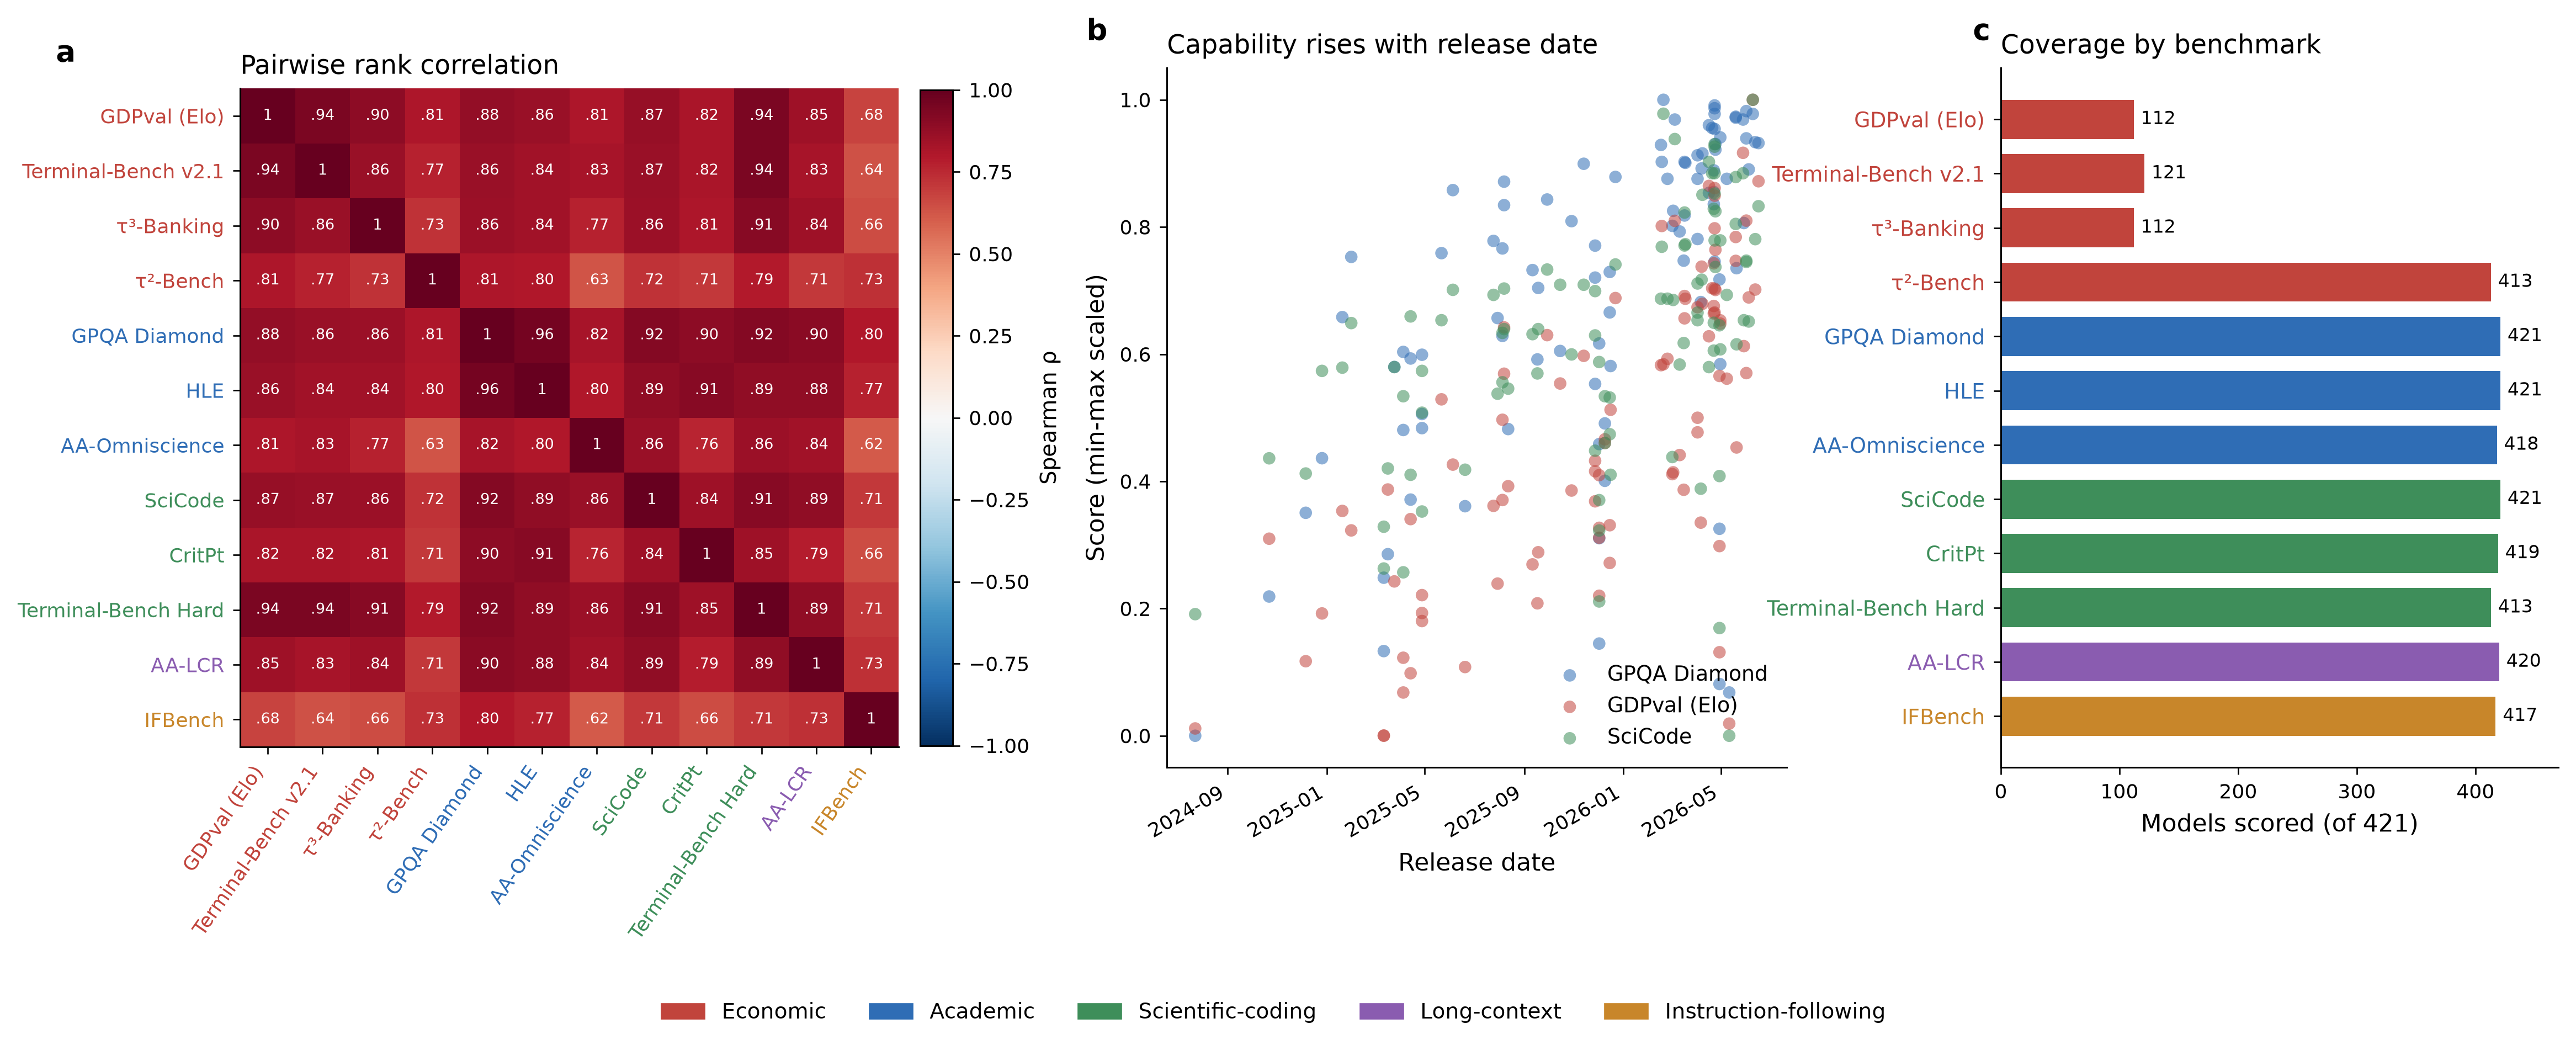
\includegraphics[width=\linewidth]{fig1_eda}
  \caption[Exploratory data analysis of the benchmark battery]{\textbf{Exploratory data analysis of the twelve-benchmark battery on the complete-case grid
  ($n=96$).} (a) Pairwise Spearman rank correlations, with benchmark labels coloured by capability
  block, where almost every pair is strongly positive. (b) Per-benchmark scores (min--max scaled) against
  model release date, showing capability rising steeply with time. (c) Coverage per benchmark across the
  421 retained models, with the four economic benchmarks (red) scored on far fewer models than the
  academic core.}
  \label{fig:eda}
\end{figure}

Missingness is also structural. Newer agentic benchmarks are simply run on fewer
models (Figure~\ref{fig:eda}c), so we use complete-case analysis on the two grids of
Section~\ref{sec:inclusion}, and we do not impute values we would then be modelling. On the complete-case
grid the Kaiser--Meyer--Olkin measure is 0.933, well above the 0.8 threshold \cite{kaiser1974}, and
Bartlett's test of sphericity is decisively rejected \cite{bartlett1950}, so factor analysis is
appropriate.

The battery is highly collinear before any modelling, with a mean off-diagonal Spearman correlation of
$\rho=0.79$ and every benchmark pair positive (Figure~\ref{fig:eda}a). The economic benchmarks correlate
with the academic core almost as strongly as with one another. A dominant general factor would produce
this near-block structure, and the structure analysis must explain it. A strong positive
manifold is equally consistent with one underlying capability and with several capabilities that improve
together over time. Distinguishing those readings is the purpose of the
residualisation in Section~\ref{sec:task1}. The temporal view makes the ambiguity concrete. Scores rise
steeply and jointly with release date (Figure~\ref{fig:eda}b), so release date is a confound for any
claim that two benchmarks measure the same thing. Because the saturation literature identifies model and
benchmark age as the strongest predictor of capability change \cite{akhtar2026}, we treat date as a
first-class nuisance variable and residualise on it before interpreting factor structure.

Beyond the correlation structure, the univariate distributions justify the transforms used later. Most benchmarks are bounded accuracies
in $[0,1]$, and several are strongly right-skewed: CritPt has Fisher skewness 3.8, HLE 1.5, and
$\tau^3$-Banking 0.9, with scores piling up near the floor (Appendix Figure~\ref{fig:eda_dist}). Two
benchmarks are unbounded, GDPval on an Elo scale and AA-Omniscience on a penalised score, and these are
closer to symmetric. Bounded skewed accuracies motivate the logit-transform robustness check in
Section~\ref{sec:robustness}, and confirms the first-factor share is not an artefact of the raw scale.
The low-scoring tails are weak models with genuinely low scores, so we retain all rows and
address the boundedness through the transform and keep all outliers.

\section{Methods}\label{sec:methods}
The analysis runs two tasks on the same data. Task~1 is unsupervised and recovers and stress-tests the
latent capability structure with three method families, namely principal-component analysis, exploratory
factor analysis, and clustering. Task~2 is supervised and tests whether that structure has out-of-sample
predictive value, using four regression learners under a leave-one-benchmark-out protocol. All features
are per-benchmark z-standardised using training-set statistics only, and the full mathematical
derivations are collected in Appendix~\ref{app:math}.

\subsection{Task 1: latent structure}\label{sec:task1}
Dimensionality is estimated by Horn's parallel analysis \cite{horn1965}, retaining factors whose
eigenvalue exceeds the 95th percentile of eigenvalues from random data of the same shape, with the scree
criterion \cite{cattell1966} as a visual cross-check. Parallel analysis is primary because it is the
more conservative of the two on strongly collinear data. We prefer factor analysis to a PCA-only
description because PCA components mix common and unique variance, whereas the common-factor model
separates shared capability from benchmark-specific idiosyncrasy, which is the distinction a
construct-validity question turns on.

The factor model is a maximum-likelihood exploratory factor analysis with an oblique oblimin rotation
\cite{thurstone1947}. We choose the oblique rotation because capability dimensions have no reason to
be uncorrelated\footnote{An orthogonal rotation such as varimax forces the factors to be uncorrelated. On data with a strong general factor this spreads shared variance across several artificially independent axes, which would obscure the dominance we are trying to measure.} and the residualised factors are in fact strongly correlated (Section~\ref{sec:h3}). The model represents each standardised benchmark score as a linear combination of $k$ latent factors plus a benchmark-specific uniqueness, derived in Appendix~\ref{app:math}. We report the first factor's
share of common variance as the dominance statistic, orienting every factor so higher means more
capable.

To separate a general capability from a shared time trend, each standardised benchmark is
regressed on release date, and on a subsample also on training compute, and the factor analysis is
re-fitted on the residuals. The change in the first factor's variance share measures how much of the
apparent general factor is a date artefact, directly comparable to the $72\%\rightarrow41\%$ correction
Kearns reports \cite{kearns2026}. This residualise-then-refit design is what lets the analysis
distinguish a single date-driven manifold from a truly multidimensional capability space.

Models are also clustered in factor-score space with $k$-means, Gaussian mixtures, and agglomerative
Ward linkage, the cluster count selected by silhouette \cite{rousseeuw1987} and the gap statistic
\cite{tibshirani2001gap}. Using three algorithms guards against a clustering that reflects one
algorithm's inductive bias. The benchmarks are separately clustered by correlation distance $1-\rho$
under average linkage, to test whether the economic benchmarks form a distinct branch.

\subsection{Task 2: predictive validity}\label{sec:task2}
The distinctiveness question is then recast as a forecast, asking whether a model's score on a held-out
economic benchmark can be predicted from its behaviour on the others. The leave-one-benchmark-out (LOBO) protocol takes each economic benchmark as the target in turn. It predicts that target from representations of the remaining eleven on the $n=96$ complete-case grid. Success requires transfer across benchmarks without memorising a single column, which a conventional random split would not enforce. A five-rung
predictor ladder of increasing richness makes the comparison concrete: rung~(i) uses release timing and
scale only, rung~(ii) a single mean-score general index, rung~(iii) the first factor only, rung~(iv) the
$k$ factors, and rung~(v) the $k$ factors plus model covariates. The contrast of interest is
rung~(iv) or (v) against the single-index rung~(ii), because a multi-factor representation beating a
single general index out of sample would show economic capability carries information the index does not.

Each rung is fitted with four learners spanning the linear-regularised and non-linear tree families
\cite{hastie2009}, ridge \cite{hoerl1970}, elastic net \cite{zou2005}, random forest \cite{breiman2001},
and gradient boosting \cite{friedman2001}, so the ladder comparison is not confounded with a single
model class. Hyperparameters are tuned by grid search in an inner five-fold cross-validation nested
inside an outer five-fold split that supplies the reported out-of-fold error, so no test fold informs
tuning or standardisation. A single non-nested cross-validation would let tuning peek at the evaluation
folds and inflate every rung. We report both train and test RMSE and out-of-fold $R^2$.

Crucially, because the factors are estimated quantities, they are re-estimated inside the loop. The factor analysis is fitted on each training fold only. The held-out fold is projected through the training-fold Thurstone factor-score weights $W = R^{-1}\Lambda$ (Appendix~\ref{app:scores}) and re-oriented by the
training-fold mean index. This prevents the factor construction from ever seeing the models it is
evaluated on, a leakage path a naive fit-on-all-data pipeline would silently open.

For each economic target we compute $\Delta\mathrm{MSE} = \mathrm{MSE}(\text{single index}) -
\mathrm{MSE}(k\ \text{factors})$, so that positive values favour the multi-factor representation. A 95\%
confidence interval is obtained by bootstrap resampling the pooled out-of-fold errors \cite{efron1993}
with $B=2000$ replicates. Hypothesis H4 is supported when the pooled interval excludes zero and a
majority of the four economic targets individually favour the multi-factor model. The complete
leave-one-benchmark-out procedure, with the leakage-safe factor re-estimation inside every fold, is
stated in full as Figure~\ref{alg:lobo} in Appendix~\ref{app:algorithm}.

\subsection{Hypotheses and pre-specified tests}\label{sec:hypotheses}
The design fixes four hypotheses with quantitative thresholds before analysis, calibrated to the
$72\%\rightarrow41\%$ result of Kearns \cite{kearns2026}. H1, dominance, holds that the first factor
carries more than 50\% of common variance. H2, the date artefact, has two parts, the first being that
the dominant factor's release-date $R^2$ is at least 0.30 and is the strongest of the factors, and the
second that residualising on date lowers the first factor's share by at least fifteen percentage points.
H3, economic distinctiveness, holds that after residualisation the four economic benchmarks load at
least 0.40 on a common factor and exceed their cross-loadings. H4, predictive validity, holds that the
multi-factor representation's $\Delta\mathrm{MSE}$ confidence interval excludes zero. We report every
outcome, including H2(ii), which is indistinguishable from its threshold once uncertainty is attached,
and H3, whose registered retention clause is not met.

The study's positionality and directionality, covering factor sign orientation, the direction of residualisation, the pre-fixed sign of the predictive contrast, and the two sampling threats to validity, are set out in Appendix~\ref{app:positionality}.

\subsection{Evaluation metrics and model selection}\label{sec:metrics}
The two tasks are evaluated with metrics matched to their aims. For the unsupervised structure task the
primary quantities are the first-factor communal-variance share for dominance, each factor's
release-date fit for temporal confounding, and the residualised loading pattern for distinctiveness,
with model adequacy checked beforehand by the Kaiser--Meyer--Olkin index and Bartlett's test. The number
of factors is chosen by parallel analysis, as information criteria over-retain on
strongly collinear data. The primary count is $k=1$, returned by
parallel analysis, the Kaiser rule, and the scree elbow. The Bayesian information criterion alone prefers
$k=4$, which we treat as over-retention. The three-factor solution used to probe economic distinctiveness
is selected by none of these criteria. It is an exploratory over-extraction that asks whether an economic
block would separate when more factors than the data support are forced out, and the choice of
three is a documented deviation from the pre-registered plan (Appendix~\ref{app:deviations}). The
predictive conclusion does not hinge on it. Sweeping the $k$-factor predictor over $k \in \{2,3,4,5\}$
beats the single index at every count with all bootstrap intervals excluding zero, and the gain grows
with $k$ (Appendix~\ref{app:robust}). At rung (iv), Task~2's $k$-factor predictor
denotes this same three-factor solution. For the supervised task the objective is mean squared error on standardised targets, reported as root
mean squared error so that it stays on the target's own scale and remains comparable across rungs and
targets. Threshold metrics such as ROC and its area do not apply. Neither task is binary
classification. Model selection is strictly nested. The inner cross-validation chooses hyperparameters and the best learner per rung, and the untouched outer cross-validation supplies the reported error. We report both train and test error in Table~\ref{tab:ladder} so any over-fitting of the kind the
timing-only rung shows is exposed.

\section{Results}\label{sec:results}
The four hypotheses are reported in order. Sections~\ref{sec:h1} to \ref{sec:h3} address the structure question. They cover the dominance of a single factor (H1), the extent to which it is a release-date artefact (H2), and whether the economic benchmarks form a distinct factor once that artefact is removed
(H3). Section~\ref{sec:clustering} corroborates the structure with clustering, Section~\ref{sec:h4}
turns to prediction (H4), Section~\ref{sec:explain} opens the best model with explainability and named
error analysis, and Section~\ref{sec:robustness} collects the robustness checks. Each hypothesis is
adjudicated against its pre-registered threshold, and the outcome is reported regardless of direction.

\subsection{Dominance of a single factor (H1)}\label{sec:h1}
Every dimensionality diagnostic points to a dominant capability axis. The first principal component
alone accounts for 79.4\% of total score variance, and parallel analysis retains a single factor, since
only the first observed eigenvalue of 9.53 exceeds its random-data 95th percentile of 1.79 while the
second, at 0.91, already falls below (Appendix Figure~\ref{fig:scree}). In the maximum-likelihood factor
analysis the first factor holds 74.5\% of common variance, above the 50\% dominance threshold and close
to the 72\% Kearns reports on a different leaderboard \cite{kearns2026}, so H1 is supported. The share is robust
to the correlation measure, since a rank-based factor analysis gives 94.5\% and a logit-transformed one
91.8\%. The Pearson-based headline is therefore the conservative choice (Section~\ref{sec:robustness}).

\subsection{A date-driven artefact (H2)}\label{sec:h2}
Having established a dominant factor, we next ask whether it reflects stable capability or the passage of
time. The factor's scores track model release date with a logistic-fit $R^2$ of 0.505, the strongest of
the three factors against 0.364 and 0.286, so H2(i) is supported and the leading axis of ``capability''
is substantially a time trend. Consequently, residualising
every benchmark on release date and re-fitting lowers the first factor's common-variance share from
74.5\% to 59.6\% (Figure~\ref{fig:loadings}c), a drop of 14.9 percentage points, so date alone accounts
for about a fifth of the general factor. This point estimate falls just short of the pre-registered fifteen-point threshold. A bootstrap over
models puts a 95\% interval of $[-5.3, +32.7]$ around it. On the primary grid the drop is therefore
indistinguishable both from zero and from the threshold, and we report H2(ii) as not met on the point
estimate without moving the line after seeing the result.

However, the verdict depends on the unit of analysis, and the main text should say so, leaving nothing to the
appendix alone. Under the registered base-model unit, which keeps one row per model, the drop is 24.1 points
and clears the threshold. Under the deviated configuration-level primary it is 14.9 points and fails. On
the 58-model compute-known subsample, date alone gives 16.5 points and also clears it. Two of the
three specifications pass. We keep the failing configuration-level specification as primary, since it is
the more conservative reading. The confirmation of a temporal confound then rests on the subsample and the
deduplicated grid, and does not rest on the primary grid alone. The residual 59.6\% share is what any downstream
capability claim must contend with.

Moreover, adding training compute to the residualisation does not deepen the correction. On the compute-known
subsample the date-only drop is 16.5 points, and the joint date-plus-compute drop is smaller at 9.3
points. That a covariate shrinks the correction is an anomaly, and the likely mechanism is
collinearity between release date and compute on this small subsample. Later models are also larger, so
regressing on both splits shared variance between two correlated predictors and leaves a smaller residual
movement. We read the result as compute adding little beyond date. The date effect stands.

\begin{figure}[htbp]
  \centering
  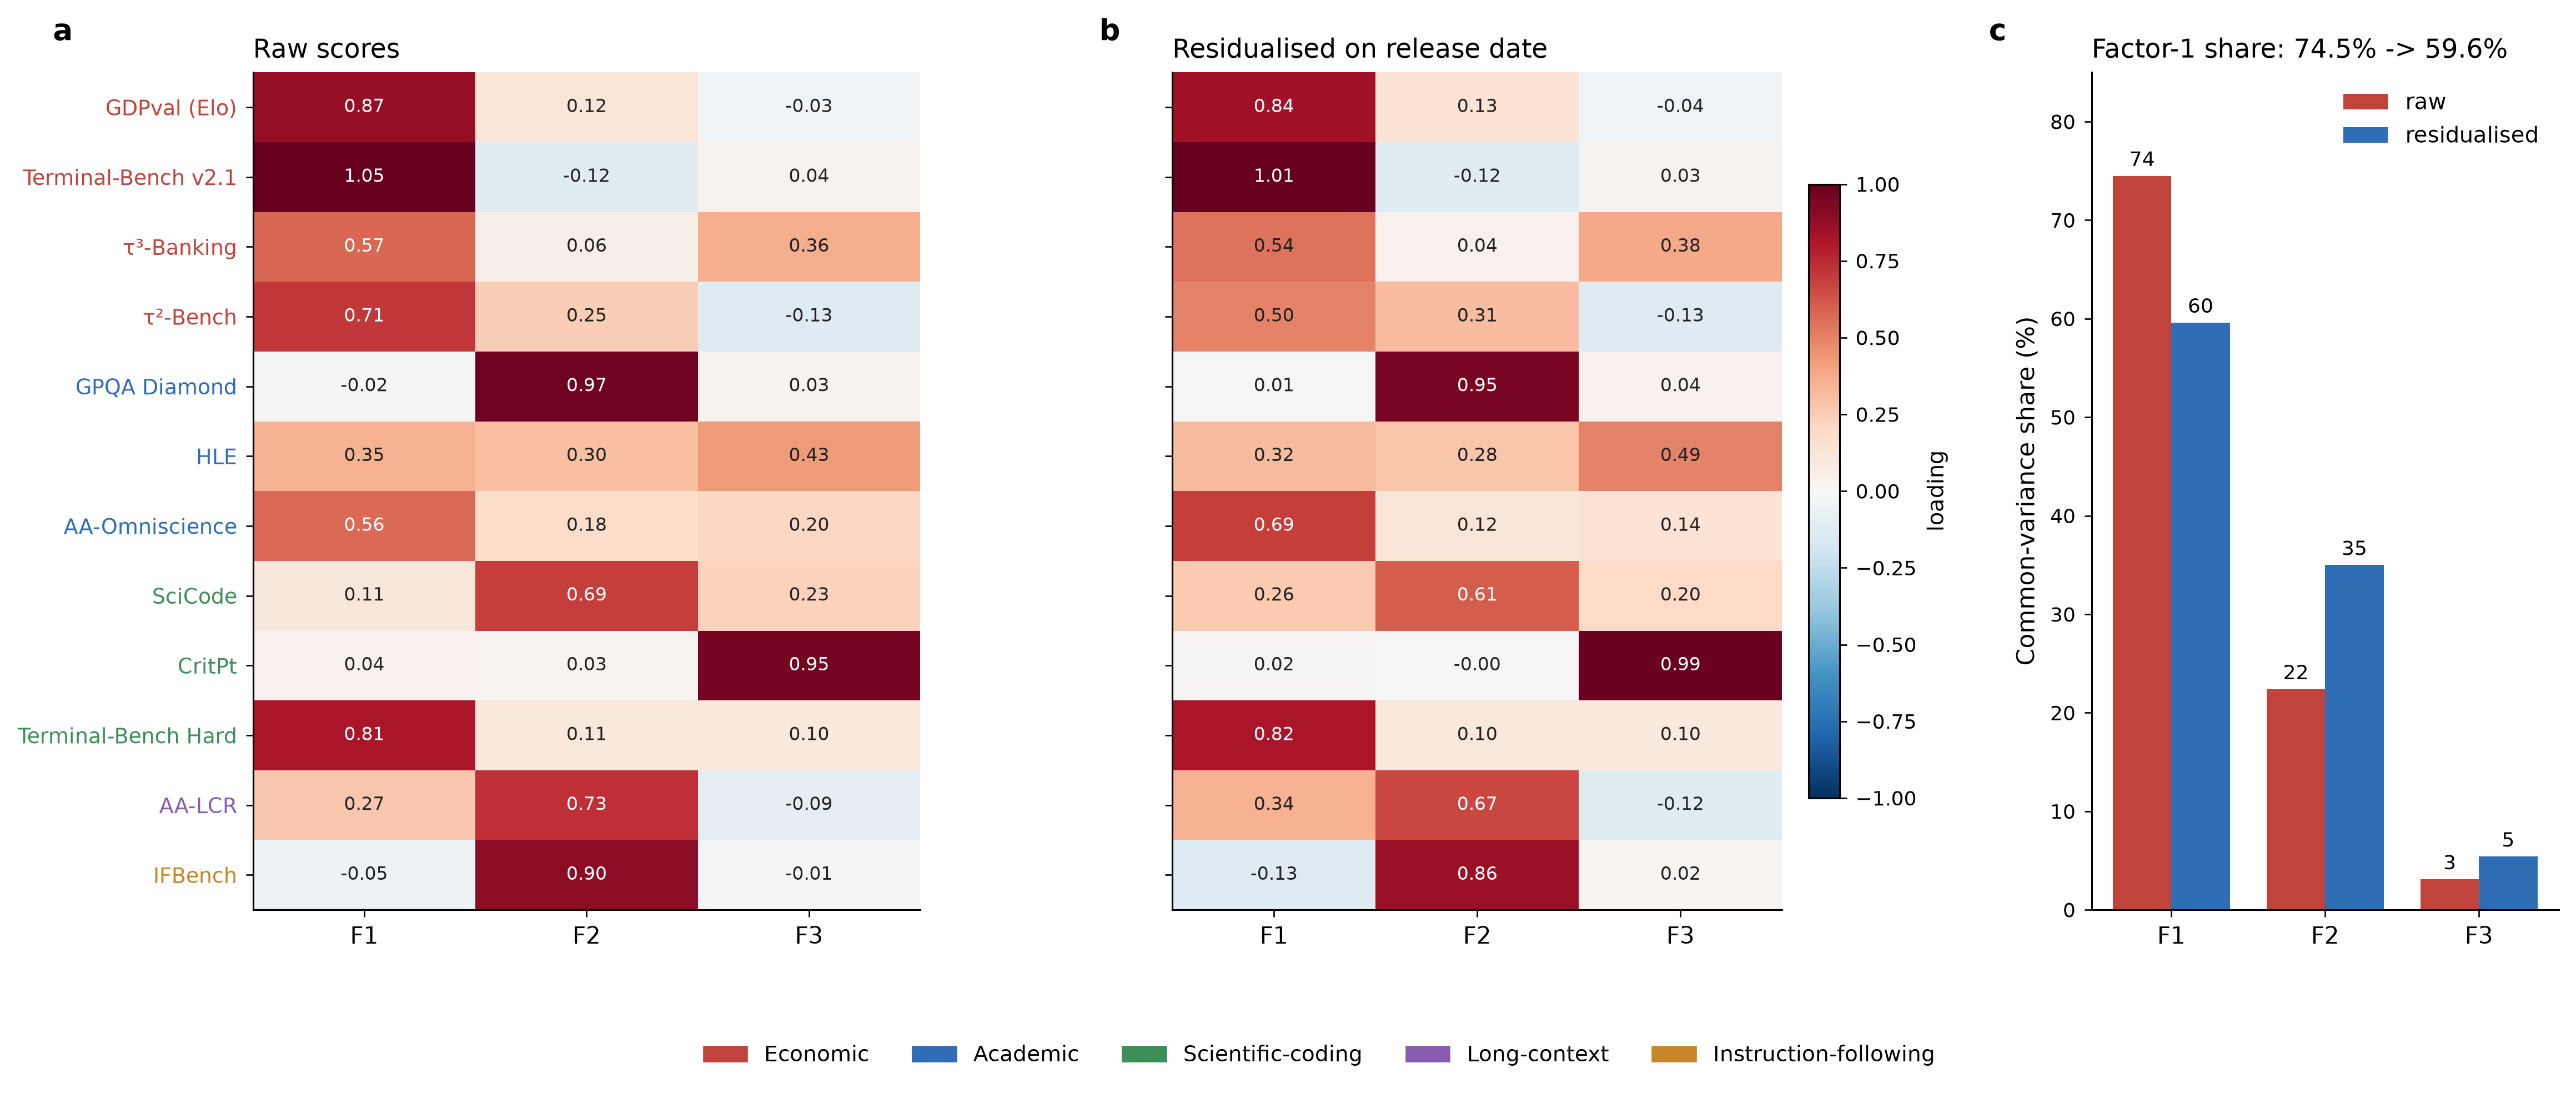
\includegraphics[width=\linewidth]{fig2_loadings}
  \caption[Factor loadings, raw and date-residualised]{\textbf{Factor loadings from the three-factor oblimin exploratory factor analysis.}
  (a) On raw scores the economic benchmarks (bold) load together with the academic core on the leading
  factor. (b) After residualising on release date, the economic benchmarks concentrate on their own
  factor F1, with a largest economic cross-loading of 0.38. (c) The first factor's
  common-variance share falls from 74.5\% to 59.6\% under residualisation, a 14.9-point drop.}
  \label{fig:loadings}
\end{figure}

\subsection{Economic distinctiveness (H3)}\label{sec:h3}
Having removed the temporal confound, we next test whether the economic benchmarks form a distinct
factor. The registered test for H3 conjoins two conditions. Parallel analysis must retain a factor, and that
factor's loadings must concentrate discriminantly on the economic block. These two conditions are not
jointly met, and we report H3 as not supported as registered. Parallel analysis on the residualised
data retains a single factor, and in that one-factor solution there is no block to separate. The
discriminant separation appears only when three factors are extracted, an extraction that the
dimensionality rule does not endorse. Holding H3 to its registration in the same way H2(ii) was held to
its 15-point line, the retention clause fails, and the pre-registered negative-result clause applies.
Under a three-factor over-extraction the economic block does separate, and we report that
pattern as exploratory. All four economic benchmarks load at least 0.40 on a single factor, F1, with
GDPval at 0.84, Terminal-Bench v2.1 at 1.01, $\tau^3$-Banking at 0.54, and $\tau^2$-Bench at 0.50,
against a largest economic cross-loading of 0.38 (Table~\ref{tab:loadings}). The mean absolute F1
loading is 0.72 for economic benchmarks versus 0.32 for the rest. The three factors are strongly
correlated, at 0.67 between F1 and F3 and 0.72 between F2 and F3, so an oblique rotation is
appropriate and why the separation is better read as a secondary refinement of one dominant axis, well short of
independent dimensions. Bootstrap intervals on the economic loadings are wide, spanning 0.10 to 0.78 for
$\tau^2$-Bench and 0.44 to 0.99 for GDPval, so the exploratory pattern is suggestive though loosely estimated. The economic factor is rescued from being an over-extraction artefact by out-of-sample
transfer. As Section~\ref{sec:h4} shows, the three-factor representation predicts held-out economic scores better than a single index. Out-of-sample transfer is a stronger dimensionality argument than an in-sample retention rule, so we let the predictive test carry the claim
the structural test cannot.

\begin{table}[!tb]
\centering
\caption[Residualised three-factor loadings]{\textbf{Residualised (date-partialled) three-factor oblimin loadings,} economic benchmarks in
bold. F1 is an agentic and work-realistic factor, F2 an academic-knowledge factor, F3 a
physics and hard-reasoning factor. All four economic benchmarks load highest on F1 with small
cross-loadings.}
\label{tab:loadings}
\small
\begin{tabular}{@{}lrrr@{}}
\toprule
Benchmark & F1 & F2 & F3 \\
\midrule
\textbf{GDPval (Elo)} & \textbf{0.84} & 0.13 & -0.04 \\
\textbf{Terminal-Bench v2.1} & \textbf{1.01} & -0.12 & 0.03 \\
\textbf{$\tau^3$-Banking} & \textbf{0.54} & 0.04 & 0.38 \\
\textbf{$\tau^2$-Bench} & \textbf{0.50} & 0.31 & -0.13 \\
GPQA Diamond & 0.01 & 0.95 & 0.04 \\
HLE & 0.32 & 0.28 & 0.49 \\
AA-Omniscience & 0.69 & 0.12 & 0.14 \\
SciCode & 0.26 & 0.61 & 0.20 \\
CritPt & 0.02 & -0.00 & 0.99 \\
Terminal-Bench Hard & 0.82 & 0.10 & 0.10 \\
AA-LCR & 0.34 & 0.67 & -0.12 \\
IFBench & -0.13 & 0.86 & 0.02 \\
\bottomrule
\end{tabular}
\end{table}

\subsection{Clustering of models and benchmarks}\label{sec:clustering}
Because a factor model can impose structure that the raw data do not support, we sought an independent check, and clustering corroborates the low dimensionality without assuming a factor model at all. Grouping models in factor-score space, all three
algorithms prefer $k=2$ by silhouette, at 0.480 for $k$-means, 0.499 for agglomerative, and 0.467 for
the Gaussian mixture (Appendix Figure~\ref{fig:clusters}b). The gap statistic increases monotonically in $k$ and identifies no interior optimum, so it is inconclusive on data with a strong general factor and we do not rely on it. The
two clusters mark capability tiers along one axis of overall strength. A larger, earlier, lower-scoring group
of 302 models, with median release 2025-09 and mean Intelligence Index 13.7, is separated from a
smaller, newer, higher-scoring group of 107 models, with median release 2026-03 and mean index 37.1.
Models separate by how much capability they have, along the same date-driven axis. They do not separate by which kind
they have (Appendix Figure~\ref{fig:clusters}a). Clustering the benchmarks by correlation distance places ten of
twelve, including three of four economic benchmarks, in one block, with $\tau^2$-Bench and IFBench
branching separately (Appendix Figure~\ref{fig:dendro}).

\FloatBarrier
\subsection{Predictive validity (H4)}\label{sec:h4}
However, structural separation alone does not make the economic factor useful, so we ask whether it predicts
held-out economic performance better than a general index. Across the predictor ladder a single
mean-score index is already a strong baseline (economic-block test RMSE 0.474, $R^2$ 0.771), yet the
$k$-factor representation improves on it to RMSE 0.433 and $R^2$ 0.808, and adding covariates does not
help further (Table~\ref{tab:ladder}, Figure~\ref{fig:pred}a). The first factor alone predicts poorly at
RMSE 0.950, locating the economic signal in the secondary factors, where the over-extraction placed
it. Bootstrapping $\Delta\mathrm{MSE}$ over the pooled out-of-fold errors gives a pooled improvement of
$+0.037$ with a 95\% interval of $[+0.019, +0.055]$. Because that resample includes near-duplicate
settings of the same base model, we re-run it on the deduplicated grid of 89 distinct models, where the
improvement is $+0.038$ with $[+0.020, +0.056]$ (Appendix~\ref{app:robust}). This model-level bootstrap
carries the inference. Three of the four economic benchmarks improve individually, GDPval by $+0.026$
with $[+0.010, +0.044]$, Terminal-Bench v2.1 by $+0.028$ with $[+0.001, +0.056]$, and $\tau^3$-Banking by
$+0.056$ with $[+0.008, +0.103]$, while $\tau^2$-Bench's interval includes zero
(Table~\ref{tab:h4}, Figure~\ref{fig:pred}b). The per-target mean of $+0.031$ is reported as a descriptive
spread, since a percentile interval over four positive means cannot include zero by construction. H4 is
therefore supported by the pre-registered rule of a pooled interval excluding zero with a majority of
targets favouring the multi-factor model. The effect is nonetheless modest. An improvement of 0.037 sits
on top of a single index that already explains 77\% of economic-block variance, so the multi-factor gain
is incremental, and it does not transform the model ranking. It survives leave-one-benchmark-out validation, and rewards
transfer across constructs and penalises memorisation. The one exception, $\tau^2$-Bench, has the widest
interval, so its null reflects limited coverage as much as an absence of signal.

\begin{figure}[!tb]
  \centering
  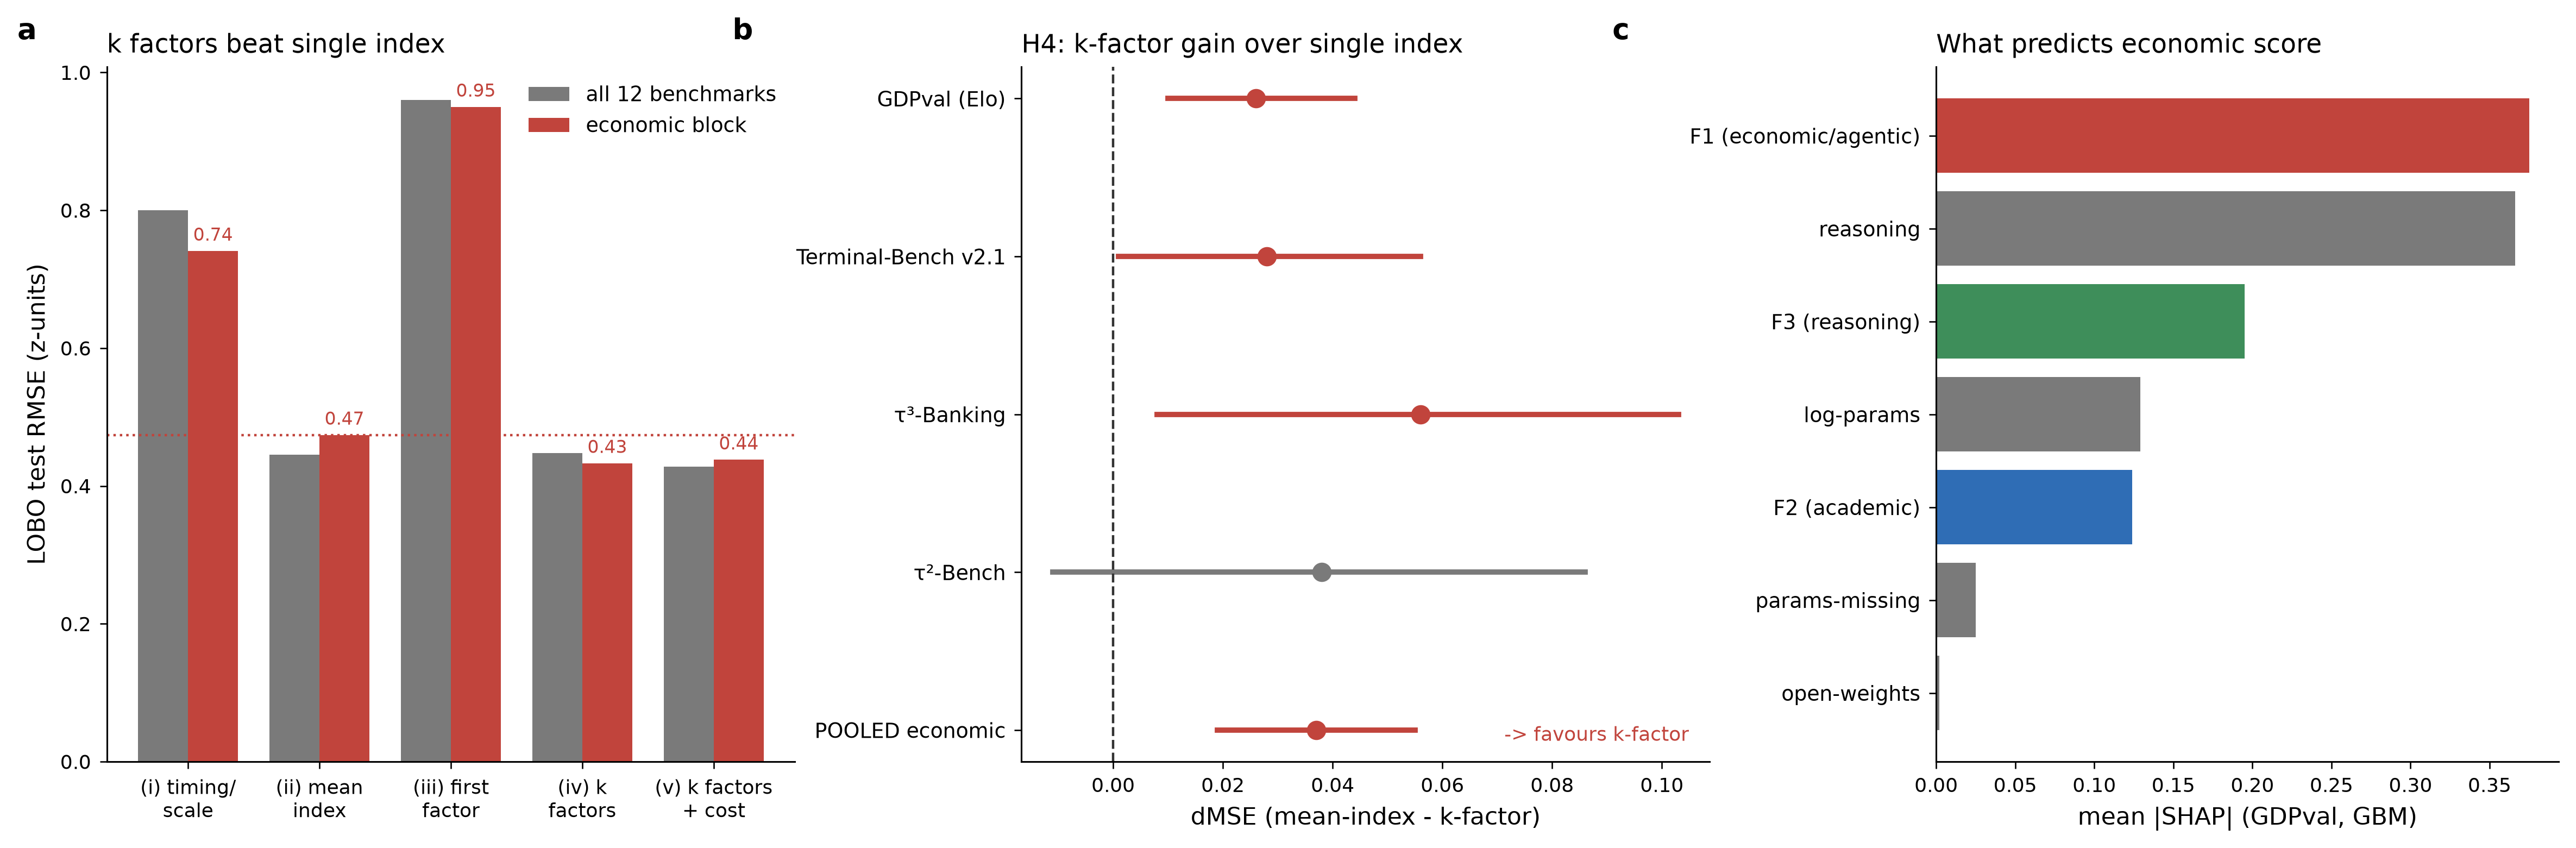
\includegraphics[width=\linewidth]{fig4_prediction}
  \caption[Predictive validity under the LOBO protocol]{\textbf{Predictive validity under the LOBO protocol.} (a) Test RMSE by predictor-ladder rung,
  for the economic block (red) and all twelve targets (grey). The $k$-factor rungs beat both the single
  index and the first-factor-only rung. (b) Bootstrap $\Delta\mathrm{MSE}$ (single index minus $k$
  factors) with 95\% intervals, where positive favours the multi-factor representation. (c) SHAP
  importances for the GDPval model, showing the agentic factor F1 and the reasoning flag dominating.}
  \label{fig:pred}
\end{figure}

\begin{table}[!tb]
\centering
\caption[Predictor-ladder cross-validated errors]{\textbf{Predictor-ladder cross-validated errors (economic block).} Train and test RMSE are on
standardised targets and test $R^2$ is out-of-fold. The best learner per rung is shown. The $k$-factor
rungs (iv, v) achieve the lowest test error. Errors are pooled over the five outer folds; the uncertainty
on the key rung~(ii)-versus-(iv) contrast is the bootstrap $\Delta\mathrm{MSE}$ interval in
Table~\ref{tab:h4}, which excludes zero.}
\label{tab:ladder}
\small
\begin{tabular}{@{}llrrr@{}}
\toprule
Rung & Best learner & Train RMSE & Test RMSE & Test $R^2$ \\
\midrule
(i) timing / scale & random forest & 0.521 & 0.741 & 0.459 \\
(ii) mean index & ridge & 0.463 & 0.474 & 0.771 \\
(iii) first factor & elastic net & 0.933 & 0.950 & 0.110 \\
(iv) $k$ factors & ridge & 0.410 & 0.433 & 0.808 \\
(v) $k$ factors + covariates & ridge & 0.391 & 0.438 & 0.800 \\
\bottomrule
\end{tabular}
\end{table}
\begin{table}[!tb]
\centering
\caption[H4 bootstrap predictive-validity test]{\textbf{H4 bootstrap} $\Delta\mathrm{MSE} = \mathrm{MSE}(\text{mean index}) -
\mathrm{MSE}(k\ \text{factors})$, $B=2000$; positive favours the multi-factor representation. Intervals
that exclude zero are marked $\checkmark$.}
\label{tab:h4}
\small
\begin{tabular}{@{}lrrc@{}}
\toprule
Target & $\Delta\mathrm{MSE}$ & 95\% CI & Excl.\ 0 \\
\midrule
GDPval (Elo) & +0.026 & [+0.010, +0.044] & $\checkmark$ \\
Terminal-Bench v2.1 & +0.028 & [+0.001, +0.056] & $\checkmark$ \\
$\tau^3$-Banking & +0.056 & [+0.008, +0.103] & $\checkmark$ \\
$\tau^2$-Bench & +0.038 & [-0.011, +0.086] &  \\
\textbf{Pooled economic} & \textbf{+0.037} & \textbf{[+0.019, +0.055]} & $\checkmark$ \\
\bottomrule
\end{tabular}
\end{table}

\FloatBarrier
\subsection{Explainability and error analysis}\label{sec:explain}
To interpret the predictive gain, we examine the best model on the largest economic target. GDPval predicted by a $k$-factor ridge with
out-of-fold $R^2$ 0.88, permutation importance and SHAP attribution \cite{lundberg2017} agree that the
agentic factor F1 is the dominant predictor, followed by the reasoning flag and the hard-reasoning
factor F3, with scale and open-weights status contributing little (Figure~\ref{fig:pred}c). The
diagnostics are clean, with the predicted-versus-observed plot lying on the identity line and residuals
showing no systematic trend (Appendix Figure~\ref{fig:diag}a,b). The largest residuals are interpretable outliers.
They include a non-reasoning variant of a frontier model that outperforms its
economic prediction, Grok 4.3 Non-reasoning at $+1.14$, and two models that under-perform theirs
(Appendix Figure~\ref{fig:diag}c), a pattern consistent with GDPval rewarding agentic behaviour that the other
benchmarks capture only indirectly.

\subsection{Robustness}\label{sec:robustness}
Finally, the headline structure is stable under design perturbations. Full tables and a deviations-from-design
account appear in Appendix~\ref{app:deviations} and~\ref{app:robust}. The most
consequential check is the registered configuration-versus-deduplication comparison. Collapsing to one
row per base model guards against near-duplicate configurations inflating correlations. It raises the
first-factor share to 90.2\% and the date-residualisation drop to 24.1 points, so the configuration-level
analysis is the conservative choice. Replacing Pearson with rank-based or logit-transformed correlations raises
the first-factor share to 94.5\% and 91.8\%, so H1 is not an artefact of the correlation
metric. On the compute-known subsample the date-only residualisation drops the share by 16.5 points, and
adding log-compute gives a smaller drop. The predictor ladder's ordering,
with the single index strong, the first factor alone weak, and the $k$ factors best, holds on both the
economic block and all twelve targets (Table~\ref{tab:ladder}). Selected hyperparameters (Table~\ref{tab:hyper}) are pluralities across targets, and the H4 verdict does not depend on the exact regularisation strength.

\section{Discussion and conclusion}\label{sec:discussion}
The two tasks answer the question in the title. The frontier benchmark battery is governed by one
dominant capability axis, a first factor holding 74.5\% of common variance. However, that axis is
substantially a release-date artefact. Models improve on everything at once as they get newer, and
partialling date out removes about a fifth of the general factor. Economic benchmarks are
not a separate kind of capability in the raw data. They sit inside the general cloud and separate into
their own factor only after the temporal axis is removed, and only under an over-extraction that a
strict dimensionality rule would not endorse. The secondary economic factor still carries out-of-sample
information, predicting held-out economic scores better than a single general index on three of four
benchmarks. The registered negative-result clause anticipated this outcome. Economic validity is
therefore limited. A date-driven progress factor accounts for most of the economic signal, and the
benchmarks add a modest increment beyond it.

The reading matters for how leaderboards should be used. A single intelligence index captures most of
what distinguishes models and is a defensible first-order summary. The residual economic signal is the
part most relevant to claims about real-world professional value, so reporting economic benchmarks
separately is justified. However, small economic-benchmark gaps between contemporaneous frontier models
call for caution. Most of the apparent spread is the shared time trend and carries little distinct
economic ability. The evidence reinforces the broader call for psychometric scrutiny of AI benchmarks
\cite{bean2025,kearns2026} and the warning that temporal effects are a first-order confound
\cite{akhtar2026}.

Moreover, the result suggests how new economic benchmarks should be validated. When most of the spread on a
benchmark is the shared date trend, the benchmark's value for distinguishing contemporaneous models
depends on the variance it adds once that trend is removed. A builder who wants to show that a new
economic suite measures something distinct can apply the two tests here directly. Among models released
in the same window, check that the benchmark's residualised loading separates from the general factor
and that it improves out-of-sample prediction of held-out economic tasks. This adds a predictive lens to
the review-based \cite{bean2025} and saturation-based \cite{akhtar2026} approaches.

\subsection{Limitations}\label{sec:limitations}
Four limitations bound the claims. The design is exploratory, so it fits no confirmatory measurement model, and the economic
factor appears only under an over-extraction relative to parallel analysis, so a pre-registered
confirmatory model on fresh data would test it more strictly. The analysis is observational. The residualisation identifies date as a strong correlate of the general factor, but does not establish that date causes the shared variance, since unobserved common causes such as shared training data across
contemporaneous models could produce the same pattern. Coverage is uneven, the economic benchmarks being
scored on far fewer models than the academic core, so the complete-case grid of 96 models is small and
the economic results carry wider uncertainty than the dense-grid clustering. Finally the results
describe one leaderboard on one date and will shift as new models arrive, a risk we mitigate with a
hash-pinned, fully reproducible snapshot.

Finally, the limitations map onto the work we would pursue next. The most immediate step is a
confirmatory factor analysis on a fresh leaderboard snapshot, which would test the over-extracted
economic factor against a pre-specified measurement model, moving beyond the exploratory one used here. A second
direction is to link benchmark scores to external measures of professional adoption, such as
task-completion rates in deployed settings, which would move the validity argument from internal
structure to external economic impact. Finally, the public snapshot omits per-task token and turn counts. Collecting them would let rung~(v) model cost and effort directly, replacing the proxy covariates used here and sharpening the test of whether economic capability is separable from the resources a model
spends to achieve it.

\subsection{Conclusion}\label{sec:conclusion}
Treating a frontier-model leaderboard as a psychometric measurement problem, we asked whether economic
benchmarks measure one capability or many, and the answer is neither extreme. They are dominated by a
single, largely date-driven general factor, yet they retain a small, real, and out-of-sample-predictive
economic component. Economic benchmarks earn their place on the leaderboard as a modest correction to a
general progress score, though they fall short of an independent axis of ability. We pre-register four quantitative tests. We report the near-threshold and not-supported verdicts as plainly as the confirmed ones, document every deviation from the plan, and pin every input. Throughout, we have tried to make this a
transparent and reproducible case study in the construct validity of AI evaluation.

\newpage
\phantomsection
\addcontentsline{toc}{section}{References}
\begin{thebibliography}{99}

\bibitem{bean2025} Bean, A. M., Kearns, R. O., Romanou, A., Hafner, F. S., Mayne, H., et al. (2025). Measuring what Matters: Construct Validity in Large Language Model Benchmarks. NeurIPS 2025 Datasets and Benchmarks Track.

\bibitem{kearns2026} Kearns, R. O. (2026). Quantifying construct validity in large language model evaluations. MSc thesis, Oxford Internet Institute, University of Oxford. arXiv:2602.15532.

\bibitem{akhtar2026} Akhtar, M., Reuel, A., Soni, P., Ahuja, S., et al. (2026). When AI Benchmarks Plateau: A Systematic Study of Benchmark Saturation. Preprint, Evaluating Evaluations (EvalEval) Coalition. arXiv:2602.16763.

\bibitem{reuel2026} Reuel, A., Ghosh, A., Chim, J., Tran, A., et al. (2026). Who Evaluates AI's Social Impacts? Mapping Coverage and Gaps in First and Third Party Evaluations. Preprint, Evaluating Evaluations (EvalEval) Coalition. arXiv:2511.05613.

\bibitem{thurstone1947} Thurstone, L. L. (1947). Multiple-Factor Analysis. University of Chicago Press.

\bibitem{horn1965} Horn, J. L. (1965). A rationale and test for the number of factors in factor analysis. Psychometrika, 30(2), 179-185.

\bibitem{cattell1966} Cattell, R. B. (1966). The scree test for the number of factors. Multivariate Behavioral Research, 1(2), 245-276.

\bibitem{kaiser1974} Kaiser, H. F. (1974). An index of factorial simplicity. Psychometrika, 39(1), 31-36.

\bibitem{bartlett1950} Bartlett, M. S. (1950). Tests of significance in factor analysis. British Journal of Psychology (Statistical Section), 3, 77-85.

\bibitem{rousseeuw1987} Rousseeuw, P. J. (1987). Silhouettes: a graphical aid to the interpretation and validation of cluster analysis. Journal of Computational and Applied Mathematics, 20, 53-65.

\bibitem{tibshirani2001gap} Tibshirani, R., Walther, G., \& Hastie, T. (2001). Estimating the number of clusters in a data set via the gap statistic. Journal of the Royal Statistical Society: Series B, 63(2), 411-423.

\bibitem{hoerl1970} Hoerl, A. E., \& Kennard, R. W. (1970). Ridge regression: biased estimation for nonorthogonal problems. Technometrics, 12(1), 55-67.

\bibitem{zou2005} Zou, H., \& Hastie, T. (2005). Regularization and variable selection via the elastic net. Journal of the Royal Statistical Society: Series B, 67(2), 301-320.

\bibitem{breiman2001} Breiman, L. (2001). Random forests. Machine Learning, 45(1), 5-32.

\bibitem{friedman2001} Friedman, J. H. (2001). Greedy function approximation: a gradient boosting machine. Annals of Statistics, 29(5), 1189-1232.

\bibitem{lundberg2017} Lundberg, S. M., \& Lee, S.-I. (2017). A unified approach to interpreting model predictions. Advances in Neural Information Processing Systems 30 (NeurIPS 2017), 4765-4774.

\bibitem{efron1993} Efron, B., \& Tibshirani, R. J. (1993). An Introduction to the Bootstrap. Chapman \& Hall.

\bibitem{pedregosa2011} Pedregosa, F., Varoquaux, G., Gramfort, A., Michel, V., et al. (2011). Scikit-learn: Machine Learning in Python. Journal of Machine Learning Research, 12, 2825-2830.

\bibitem{aa2026} Artificial Analysis. (2026). Artificial Analysis LLM Leaderboard and Intelligence Index. https://artificialanalysis.ai (snapshot accessed 6 July 2026).

\bibitem{epoch2026} Epoch AI. (2026). Notable AI Models (data set, CC-BY 4.0). https://epoch.ai/data/notable-ai-models.

\bibitem{hastie2009} Hastie, T., Tibshirani, R., \& Friedman, J. (2009). The Elements of Statistical Learning: Data Mining, Inference, and Prediction (2nd ed.). Springer.
\end{thebibliography}


\clearpage
\appendix
\section*{Appendix}
\addcontentsline{toc}{section}{Appendix}
\renewcommand{\thesubsection}{\Alph{subsection}}
\setcounter{subsection}{0}

This appendix collects the material that supports the main text without interrupting its argument. It
states the prediction algorithm (\ref{app:algorithm}) and the study's positionality (\ref{app:positionality}),
gives the mathematical derivations behind the factor and prediction models (\ref{app:math}), the full
coverage audit behind the inclusion rule (\ref{app:coverage}), the tuning grid (\ref{app:hyper}), the
robustness battery (\ref{app:robust}), the reproducibility and provenance record (\ref{app:provenance}),
and the supplementary figures referenced from the results (\ref{app:figures}). Each subsection opens with
a one-line statement of what it supports and where the main text relies on it.

\subsection{Leave-one-benchmark-out procedure}\label{app:algorithm}
\emph{Supports Section~\ref{sec:task2}, which describes the protocol in words.}
\begin{figure}[H]
\centering
\fbox{\parbox{0.95\linewidth}{
\small
\textbf{Procedure}\quad Leave-one-benchmark-out predictive validity with nested cross-validation\\[2pt]
\hrule
\vspace{3pt}
\textbf{Input:} standardised score matrix $Z$ (models $\times$ benchmarks), economic targets $T$, learners $L$, rungs $R$.\\[2pt]
\textbf{for} each target $t \in T$ \textbf{do}\\
\hspace*{1em} partition models into 5 outer folds\\
\hspace*{1em} \textbf{for} each outer fold $(\mathrm{train}, \mathrm{test})$ \textbf{do}\\
\hspace*{2em} fit standardisation and EFA on $\mathrm{train}$ only; form Thurstone weights $W = R^{-1}\Lambda$\\
\hspace*{2em} project $\mathrm{test}$ models through $W$; orient factors by train mean index\\
\hspace*{2em} \textbf{for} each rung $r \in R$ and learner $\ell \in L$ \textbf{do}\\
\hspace*{3em} tune $\ell$ by inner 5-fold grid search on $\mathrm{train}$; predict $\mathrm{test}$, store out-of-fold error\\
\hspace*{1em} select best learner per rung by pooled out-of-fold RMSE\\
compute $\Delta\mathrm{MSE} = \mathrm{MSE}(\text{rung ii}) - \mathrm{MSE}(\text{rung iv})$; bootstrap $B=2000$ for 95\% CI\\[2pt]
\textbf{Output:} per-target and pooled $\Delta\mathrm{MSE}$ with confidence intervals (H4).
}}
\caption[Leave-one-benchmark-out prediction procedure]{The leave-one-benchmark-out procedure with leakage-safe factor projection and nested tuning.}
\label{alg:lobo}
\end{figure}

\subsection{Positionality, directionality, and threats to validity}\label{app:positionality}
\emph{Supports Section~\ref{sec:hypotheses}, which summarises these commitments in one sentence.}
Because a factor solution is identified only up to sign, the direction of every factor is a choice we
state explicitly. We orient each factor to correlate positively with the model's mean standardised
score, so that ``higher'' always means ``more capable'' and every loading in Table~\ref{tab:loadings}
reads in the same direction. The point is not cosmetic, since an un-oriented solution could report the
same economic factor with flipped signs and invite the opposite interpretation. The direction of the
residualisation is equally deliberate. We regress scores on release date and analyse the residuals,
which asks how much benchmark co-movement remains once the release date is known, and we do not run the
reverse regression, because we make no claim that the general factor causes the calendar. Finally we fix
the sign of the predictive contrast in advance, defining $\Delta\mathrm{MSE}$ as the single-index error
minus the $k$-factor error so that a positive value favours the richer representation, and pre-register
that H4 requires this positive interval to exclude zero rather than testing the reverse direction.

Two threats to validity follow from the vantage point of the study. First, we observe only the models
that vendors chose to submit to a public leaderboard, so the sample is a convenience sample of frontier
systems and not a random draw, and the claims generalise to models on this leaderboard rather than to
all models. Second, the economic benchmarks are newer and sparser, so any economic-specific structure is
estimated from fewer observations and is more sensitive to the particular set of models that happen to
carry those scores, a limitation we quantify with the wide bootstrap intervals in Table~\ref{tab:h4}
rather than hide behind point estimates.

\subsection{Mathematical derivations}\label{app:math}
\emph{Supports Sections~\ref{sec:task1} and \ref{sec:task2}, which state the factor and prediction models
in words and defer their formal statement to here.}

\medskip
\noindent\textbf{The exploratory factor-analysis model.}
Let $\mathbf{z}\in\mathbb{R}^{p}$ be the vector of $p$ per-benchmark z-standardised scores for a model.
The common-factor model represents it as a linear combination of $k$ latent factors
$\mathbf{f}\in\mathbb{R}^{k}$ plus a benchmark-specific uniqueness $\boldsymbol{\varepsilon}$,

\[
  \mathbf{z} = \Lambda \mathbf{f} + \boldsymbol{\varepsilon},
\]

where $\Lambda\in\mathbb{R}^{p\times k}$ is the loading matrix. Assuming
$\mathrm{Cov}(\mathbf{f})=\Phi$, $\mathrm{Cov}(\boldsymbol{\varepsilon})=\Psi$ diagonal, and
$\mathrm{Cov}(\mathbf{f},\boldsymbol{\varepsilon})=\mathbf{0}$, the model implies the covariance
structure

\[
  \Sigma = \Lambda \Phi \Lambda^{\top} + \Psi .
\]

\medskip
\noindent
The parameters are estimated by maximum likelihood under multivariate normality. The dominance statistic
for H1 is computed on the unrotated solution, where the factors are orthogonal ($\Phi=I$) and each
factor's contribution to common variance is its sum of squared loadings, $\sum_{j=1}^{p}\lambda_{jm}^2$,
the $m$-th diagonal entry of $\Lambda^{\top}\Lambda$. The first factor's share of common variance is
therefore
\[
  s_1 \;=\; \frac{\sum_{j=1}^{p}\lambda_{j1}^2}{\sum_{m=1}^{k}\sum_{j=1}^{p}\lambda_{jm}^2}
        \;=\; \frac{(\Lambda^{\top}\Lambda)_{11}}{\operatorname{tr}(\Lambda^{\top}\Lambda)} .
\]
On the complete-case grid the three factors carry sums of squared loadings $7.79$, $2.34$, and $0.32$, so
$s_1 = 7.79/10.45 = 74.5\%$. This is a factor-level share, distinct from a single benchmark's communality
$\sum_{m}\lambda_{jm}^2$, which is a diagonal entry of $\Lambda\Lambda^{\top}$.

\medskip
\noindent\textbf{Oblique rotation and factor scores.}
The maximum-likelihood solution is identified only up to rotation, so we apply an oblique oblimin
rotation, which minimises a quartimin-type criterion on the loadings while allowing $\Phi\neq I$. Factor
scores are then recovered by the Thurstone regression method,

\[
  \mathbf{W} = R^{-1}\Lambda, \qquad \hat{\mathbf{f}} = \mathbf{W}^{\top}\mathbf{z},
\]

where $R$ is the sample correlation matrix. In the prediction task $\mathbf{W}$ is estimated on the
training fold only and applied to the held-out fold, which is the leakage-safe projection referenced in
Section~\ref{sec:task2}.\label{app:scores}

\medskip
\noindent\textbf{Date and scale residualisation.}
To separate general capability from a shared time trend, each standardised benchmark $z_j$ is regressed
on model release date $d$ (and, in a subsample, on log training compute),

\[
  z_j = \beta_{0j} + \beta_{1j}\, d + r_j ,
\]

and the factor model is re-fitted on the residuals $r_j$. The change in the first factor's variance
share between the raw and residualised fits, $74.5\%\rightarrow 59.6\%$, is the H2(ii) statistic.

\medskip
\noindent\textbf{Nested leave-one-benchmark-out estimator.}
For an economic target $t$, the out-of-fold error of rung $r$ is

\[
  \mathrm{MSE}_r = \frac{1}{n}\sum_{i=1}^{n}\bigl(z_{it} - \hat{z}_{it}^{(-\kappa(i))}\bigr)^{2},
\]

where $\hat{z}_{it}^{(-\kappa(i))}$ is the prediction for model $i$ from a learner trained on the outer
folds excluding the fold $\kappa(i)$ containing $i$, with hyperparameters chosen by an inner five-fold
grid search on those training folds. The predictive-validity statistic contrasts the single-index rung
against the $k$-factor rung,

\[
  \Delta\mathrm{MSE} = \mathrm{MSE}_{\text{ii}} - \mathrm{MSE}_{\text{iv}} .
\]

\medskip
\noindent\textbf{Bootstrap confidence interval.}
A 95\% interval for $\Delta\mathrm{MSE}$ is obtained by resampling the paired out-of-fold squared-error
vectors with replacement $B=2000$ times and taking the 2.5th and 97.5th percentiles of the resampled
differences. H4 is supported when this interval excludes zero.

\subsection{Benchmark battery}\label{app:battery}
\emph{Supports Section~\ref{sec:battery}, which names the battery and defers the full description here.}
\begin{table}[tb]
\centering
\caption[The twelve-benchmark battery]{\textbf{The twelve-benchmark battery, grouped by capability block,} with the construct each
targets and its coverage in the analysis snapshot (models scored, of 421 retained). Higher is better for
all; GDPval is an Elo rating, the others accuracy-type scores.}
\label{tab:battery}
\small
\begin{tabular}{@{}llr@{}}
\toprule
Benchmark & Construct measured & Coverage \\
\midrule
\multicolumn{3}{@{}l}{\textit{Economic}}\\
GDPval (Elo) & Paid professional task quality & 112 \\
Terminal-Bench v2.1 & Terminal / agentic task completion & 121 \\
$\tau^3$-Banking & Multi-step banking workflows & 112 \\
$\tau^2$-Bench & Tool-use agentic tasks & 413 \\
\multicolumn{3}{@{}l}{\textit{Academic}}\\
GPQA Diamond & Graduate-level science QA & 421 \\
HLE & Humanity's Last Exam (frontier knowledge) & 421 \\
AA-Omniscience & Broad knowledge, hallucination-penalised & 418 \\
\multicolumn{3}{@{}l}{\textit{Scientific coding}}\\
SciCode & Research-level scientific coding & 421 \\
CritPt & Physics problem solving & 419 \\
Terminal-Bench Hard & Hard terminal coding tasks & 413 \\
\multicolumn{3}{@{}l}{\textit{Long-context / instruction}}\\
AA-LCR & Long-context reasoning & 420 \\
IFBench & Instruction following & 417 \\
\bottomrule
\end{tabular}
\end{table}

\subsection{Full coverage audit}\label{app:coverage}
\emph{Supports the inclusion rule of Section~\ref{sec:inclusion};} Table~\ref{tab:coverage} reports every
candidate benchmark on the raw snapshot and the decision applied to it.

\begin{table}[htbp]
\centering
\caption[Full candidate-benchmark coverage audit]{Full candidate-benchmark coverage on the raw 548-model snapshot, with the inclusion decision.
Twelve benchmarks are primary, MMMU-Pro is demoted to sensitivity-only for sparse and multimodal
coverage, and APEX-Agents is dropped below the sixty-model floor.}
\label{tab:coverage}
\small
\begin{tabular}{@{}llrl@{}}
\toprule
Benchmark & Block & Models scored & Role \\
\midrule
GPQA Diamond & Academic & 513 & primary \\
HLE & Academic & 509 & primary \\
AA-Omniscience & Academic & 418 & primary \\
MMMU-Pro & Academic & 204 & sensitivity only \\
$\tau^2$-Bench & Economic & 428 & primary \\
Terminal-Bench v2.1 & Economic & 121 & primary \\
GDPval (Elo) & Economic & 117 & primary \\
$\tau^3$-Banking & Economic & 112 & primary \\
APEX-Agents & Economic & 26 & dropped (sparse) \\
IFBench & Instruction-following & 437 & primary \\
AA-LCR & Long-context & 441 & primary \\
SciCode & Scientific-coding & 507 & primary \\
CritPt & Scientific-coding & 422 & primary \\
Terminal-Bench Hard & Scientific-coding & 421 & primary \\
\bottomrule
\end{tabular}
\end{table}

\subsection{Hyperparameter grid and selections}\label{app:hyper}
\emph{Supports Section~\ref{sec:task2} and the robustness claim of Section~\ref{sec:robustness}} that the
H4 verdict does not hinge on a single tuning choice. The inner grid searched ridge and elastic-net
$\alpha\in\{0.03,0.1,0.3,1,3\}$ with elastic-net $\ell_1$ ratio in $\{0.2,0.5,0.8\}$, random-forest
depth in $\{4,8,\text{none}\}$ with $\{200,300\}$ trees, and gradient-boosting depth in $\{2,3\}$ with
learning rate in $\{0.05,0.1\}$. Table~\ref{tab:hyper} reports the modal selection per rung.

\begin{table}[htbp]
\centering
\caption[Modal selected hyperparameters]{Modal hyperparameters selected by the inner five-fold grid search, reported as the plurality
choice across all twelve leave-one-benchmark-out targets with the agreement count. The H4 verdict rests
on fold-averaged out-of-fold errors, not on any single setting.}
\label{tab:hyper}
\small
\begin{tabular}{@{}lllc@{}}
\toprule
Rung & Learner & Modal hyperparameters & Agreement \\
\midrule
(i) timing / scale & random forest & \texttt{max\_depth}=4, \texttt{min\_samples\_leaf}=3, \texttt{n\_estimators}=300 & 8/12 \\
(ii) mean index & ridge & \texttt{alpha}=0.03 & 6/12 \\
(iii) first factor & elastic net & \texttt{alpha}=0.03, \texttt{l1\_ratio}=0.2 & 5/12 \\
(iv) $k$ factors & ridge & \texttt{alpha}=0.03 & 6/12 \\
(v) $k$ factors + covariates & ridge & \texttt{alpha}=1 & 6/12 \\
\bottomrule
\end{tabular}
\end{table}

\subsection{Deviations from the pre-registered design}\label{app:deviations}
\emph{Supports the reproducibility claims throughout.} A study that invokes pre-registration owes the
reader an explicit account of where the delivery departed from the plan. Four departures matter. First,
the registered primary unit was one row per base model at its best default configuration; the analysis
instead uses all 421 configurations, with the deduplicated base-model dataset reported below as the
registered R1 check rather than as the primary. Second, the registered factor-count rule is parallel
analysis, which retains one factor; the three-factor solution that exhibits economic separation is a
pre-declared exploratory over-extraction, and H3 is reported as not supported under the registration in
consequence. Third, the taxonomy places Terminal-Bench Hard in scientific coding whereas the
registration grouped it with Terminal-Bench v2.1 as economic; the residualised loadings show Hard at
0.82 on the economic factor, so the assignment is genuinely contestable and the split is disclosed
rather than silently adopted. Fourth, the delivered robustness checks are not the registered suite, and
we label them distinctly below instead of renumbering a different battery onto the registered names.

\subsection{Robustness checks}\label{app:robust}
\emph{Supports Section~\ref{sec:robustness}.} We first report the one registered check that bears
directly on the deduplication concern, then the additional checks actually delivered. \textbf{Registered
R1 (configuration versus deduplicated).} We collapse the 421 configurations to one row per base model,
keeping the best default configuration as the registration specified, operationalised as the
highest-intelligence-index row for each base model after stripping reasoning, effort, and preview
suffixes from the model name. This leaves 320 base models, of which 89 carry the complete battery. On this deduplicated grid the
first-factor share rises to 90.2\% and the date-residualisation drop rises to 24.1 points, and the four
economic loadings remain above 0.40, so deduplication strengthens H1 and H2(ii) and leaves the
exploratory economic pattern intact. The configuration-level analysis is therefore the conservative
choice for the structural headline. We also re-run the H4 predictive test on this deduplicated grid,
where the bootstrap resampling unit is a distinct base model rather than a configuration. The pooled
economic-block improvement of the $k$-factor representation over the single index is $+0.038$ with a 95\%
interval of $[+0.020, +0.056]$, matching the configuration-level $+0.037$ and again excluding zero, so
the predictive gain does not depend on treating near-duplicate configurations as exchangeable. \textbf{Delivered checks C1--C6.} (C1) A rank-based factor analysis
raises the first-factor share to 94.5\%, and (C2) a logit transform of the bounded accuracy benchmarks
raises it to 91.8\%, so H1 is not a Pearson artefact. (C3) On the 58-model compute-known subsample, the
date-only residualisation drops the first-factor share by 16.5 points and adding log-compute jointly
gives a smaller 9.3-point drop, so compute does not deepen the temporal correction beyond date on the
same models. (C4) The three clustering algorithms agree on $k=2$. (C5) The predictor-ladder ordering
holds on both the economic block and all twelve targets. (C6) The dominant-factor date fit is robust to
the link function: a logistic fit gives $R^2=0.505$ against an ordinary-least-squares $R^2=0.477$, both
clearing 0.30 with the first factor ranked strongest, so H2(i) does not depend on that modelling choice.
(C7) The $k$-factor predictive advantage does not depend on the exploratory factor count. Sweeping the
rung-(iv) predictor over $k \in \{2,3,4,5\}$, the improvement over the single index is positive at every
count with a bootstrap interval excluding zero: $+0.021$ at $k=2$, $+0.037$ at the $k=3$ we use, $+0.058$
at the criterion's $k=4$, and $+0.059$ at $k=5$, with pooled test $R^2$ rising from 0.79 to 0.83 across
the range. The gain increases with $k$, so using the $k=3$ we adopt is conservative for this test
relative to the criterion's $k=4$.
The registered checks not run are R3 (FIML and MICE missingness sensitivity), R4 (replication of the
single-factor foil then correction), R5 (reasoning-effort variants as a second scale axis), and R6 (the
taxonomy swap test); each was deferred for space and is the natural next step given the deviations above,
particularly R5 and R6, which bear on the effort and taxonomy departures.

\subsection{Data provenance and reproducibility}\label{app:provenance}
\emph{Supports Section~\ref{sec:source} and the reproducibility claims throughout.} The primary data set
is the Artificial Analysis model leaderboard \cite{aa2026}, captured 2026-07-06 as a raw HTML snapshot
and pinned by the SHA-256 hash recorded in the shipped manifest
(\texttt{aa\_snapshot\_manifest.json}),
\texttt{\seqsplit{6f19f8f08befaaf14cb2d9952e379404c39f246b52d7ae4d1c2aa44795404de6}}. The Data API endpoint returned
HTTP 401 to our unauthenticated request, so the public leaderboard page was captured and the exact bytes
stored, which makes every downstream number reproducible regardless of subsequent live-page drift. The
secondary data set is Epoch AI Notable AI Models \cite{epoch2026}, released under CC-BY 4.0, used only
for the scale robustness check. Both snapshots and every result table travel with the submission bundle.
The complete pipeline is in a single notebook, \texttt{analysis.ipynb}, which regenerates all
figures and tables from the pinned inputs, and the full code and data will be released at
\url{https://github.com/louisyzhu/frontier-ai-economic-validity}.

\subsection{Supplementary figures}\label{app:figures}
\emph{Supports Sections~\ref{sec:inclusion}, \ref{sec:h1}, and \ref{sec:clustering}.}
Figure~\ref{fig:density} documents the coverage audit behind the inclusion rule, Figure~\ref{fig:clusters}
shows the model clustering, Figure~\ref{fig:diag} the GDPval regression diagnostics, Figure~\ref{fig:scree} gives the dimensionality evidence behind H1, and
Figure~\ref{fig:dendro} the benchmark-level clustering behind Section~\ref{sec:clustering}.

\begin{figure}[htbp]
  \centering
  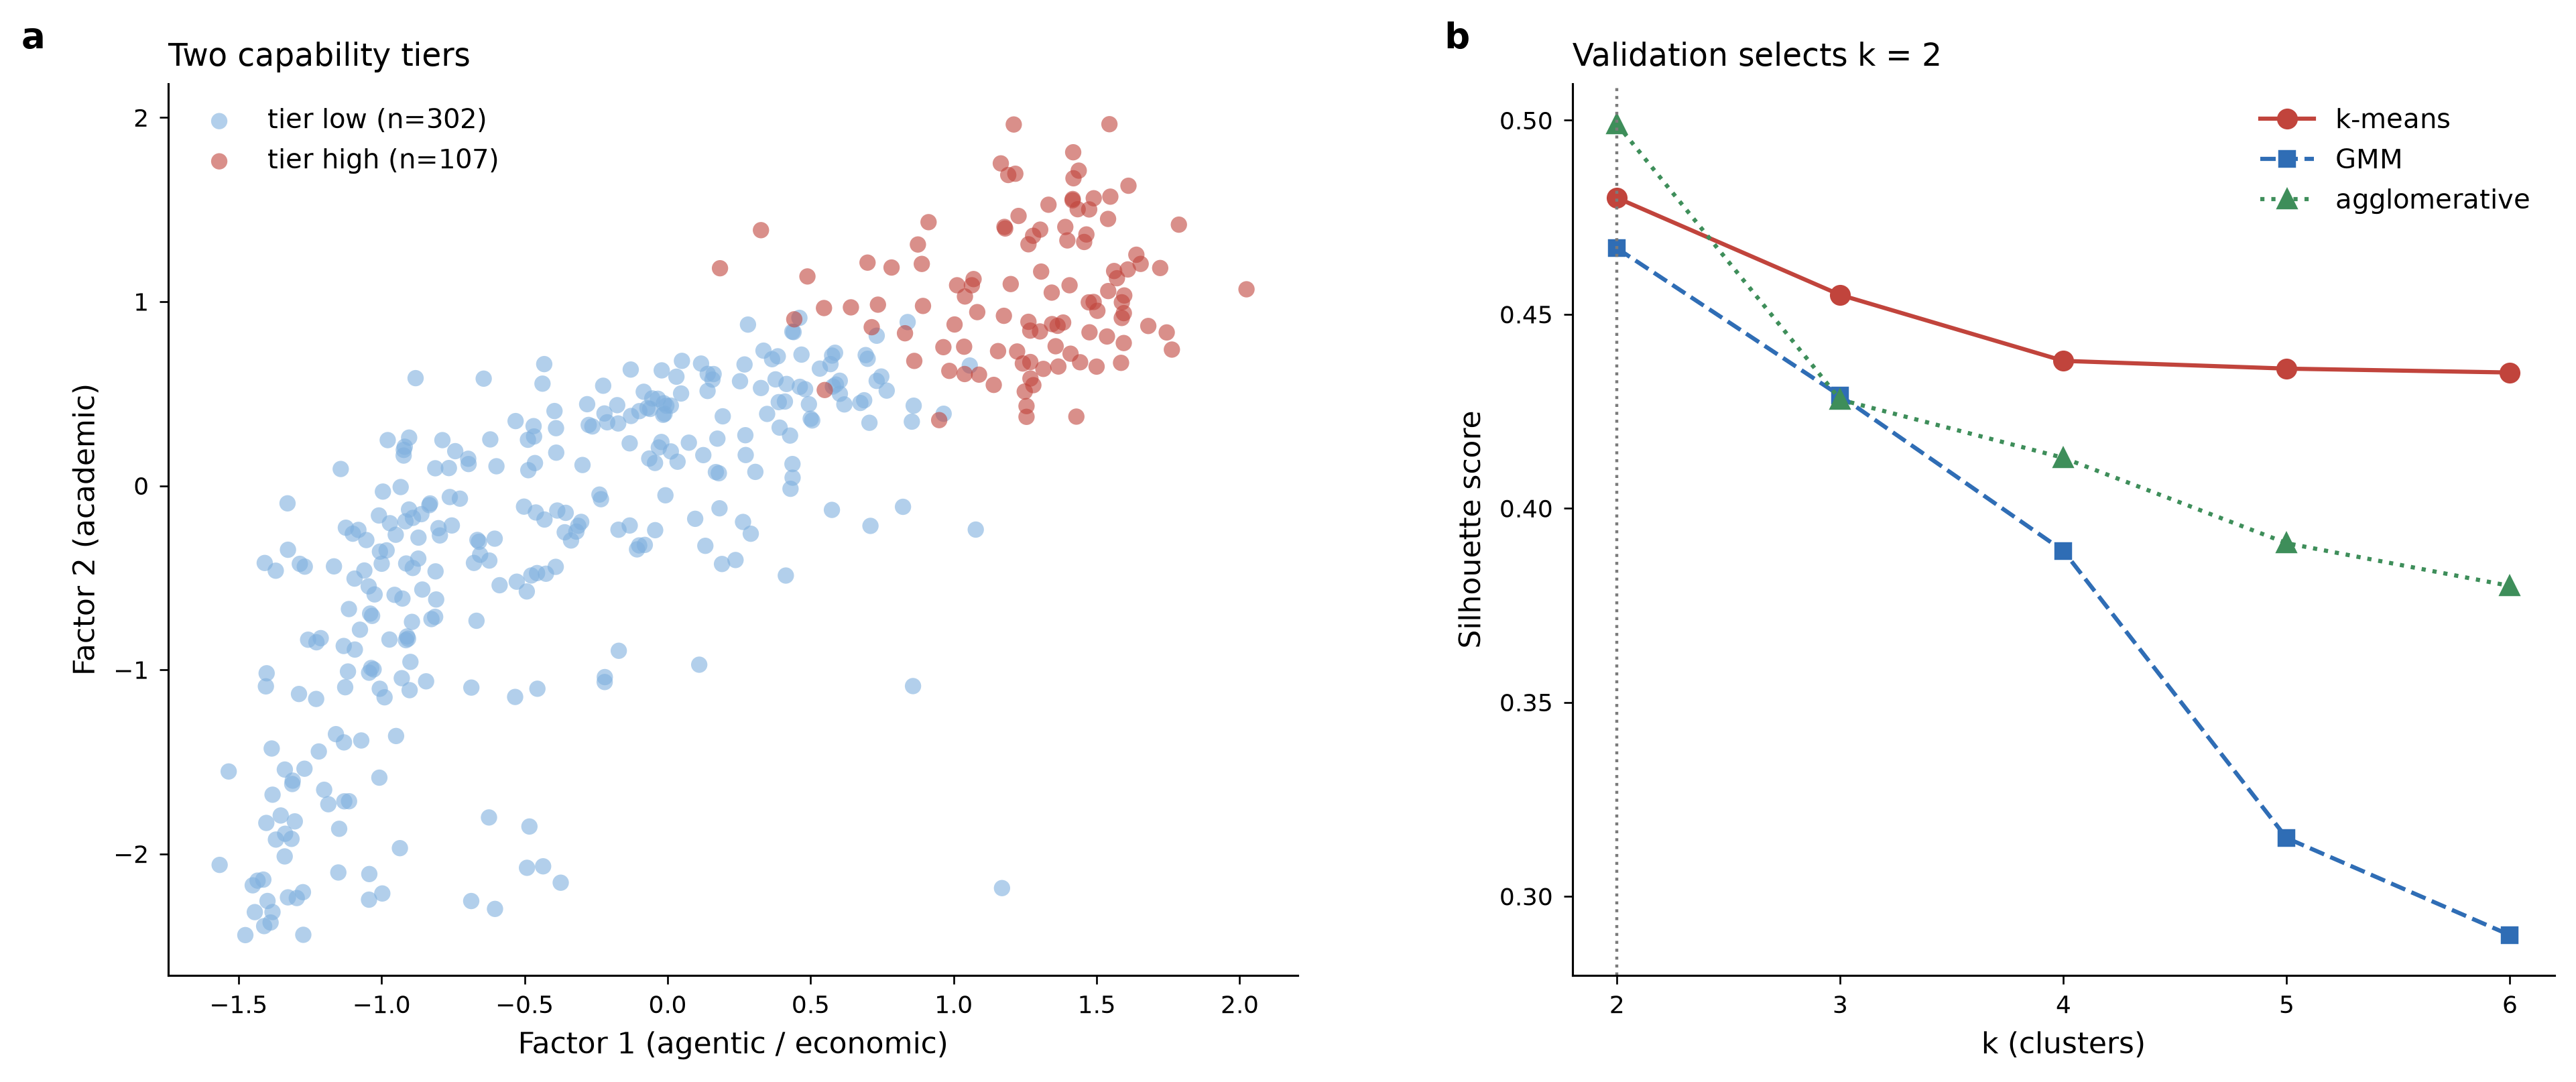
\includegraphics[width=\linewidth]{fig3_clusters}
  \caption[Model clustering into two capability tiers]{\textbf{Model clustering on the dense grid ($n=409$).} (a) Models in the space of the first
  two factors, coloured by the two-cluster agglomerative solution; the factor axes are the dense-grid
  solution fitted largely without the economic columns, so they index general capability tiers rather
  than economic type. (b) Silhouette scores by $k$ for all three algorithms agree on $k=2$.}
  \label{fig:clusters}
\end{figure}

\begin{figure}[htbp]
  \centering
  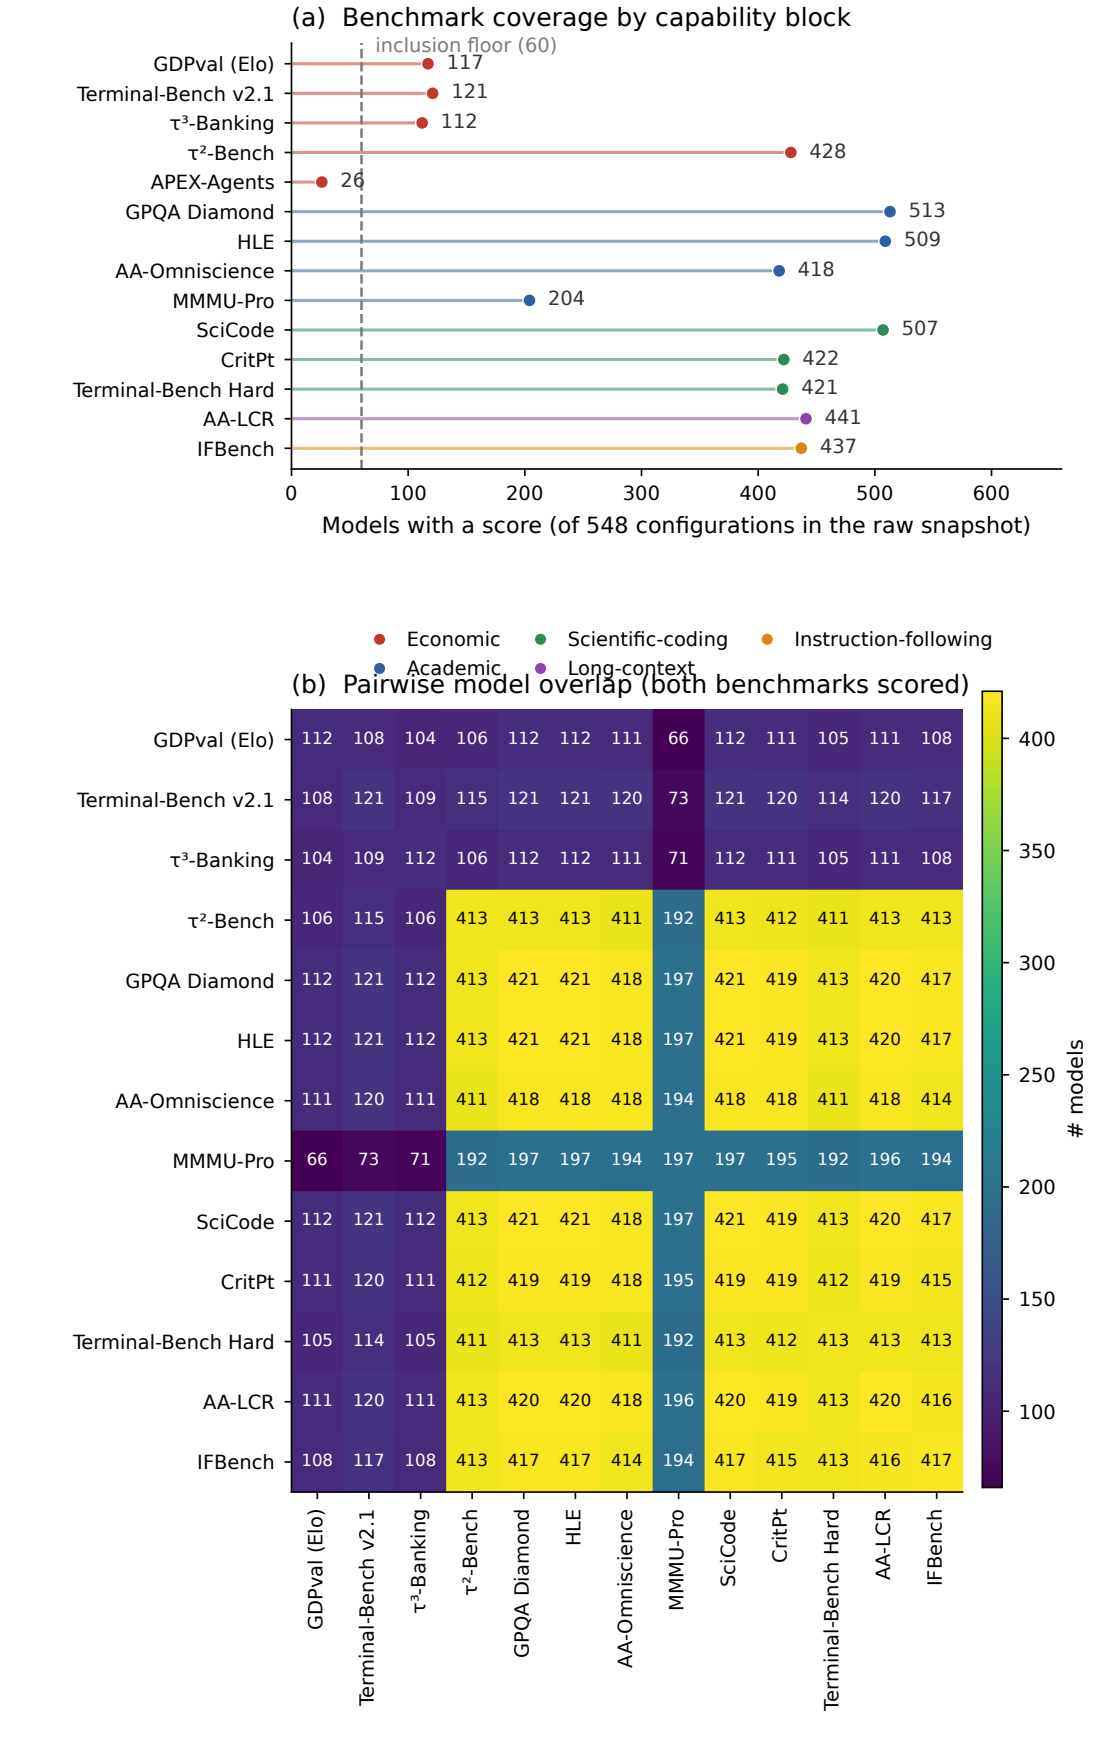
\includegraphics[width=\linewidth]{appxfig_density}
  \caption[Coverage and pairwise-overlap audit]{\textbf{Coverage audit behind the inclusion rule.}
  (a) Number of models carrying a score on each candidate benchmark, coloured by capability block, with
  the sixty-model inclusion floor marked. Four of the five economic benchmarks are retained; three of
  them (Terminal-Bench v2.1, GDPval, and $\tau^3$-Banking) are scored on only 112 to 121 models, whereas
  $\tau^2$-Bench and the academic core are each scored on four hundred or more. APEX-Agents, with 26
  models, falls below the floor and is dropped. (b) Pairwise counts of models scored
  on both benchmarks in a pair, which set the effective sample size for every correlation in the study.
  This is the evidence for the two-grid design of Section~\ref{sec:inclusion}.}
  \label{fig:density}
\end{figure}

\begin{figure}[htbp]
  \centering
  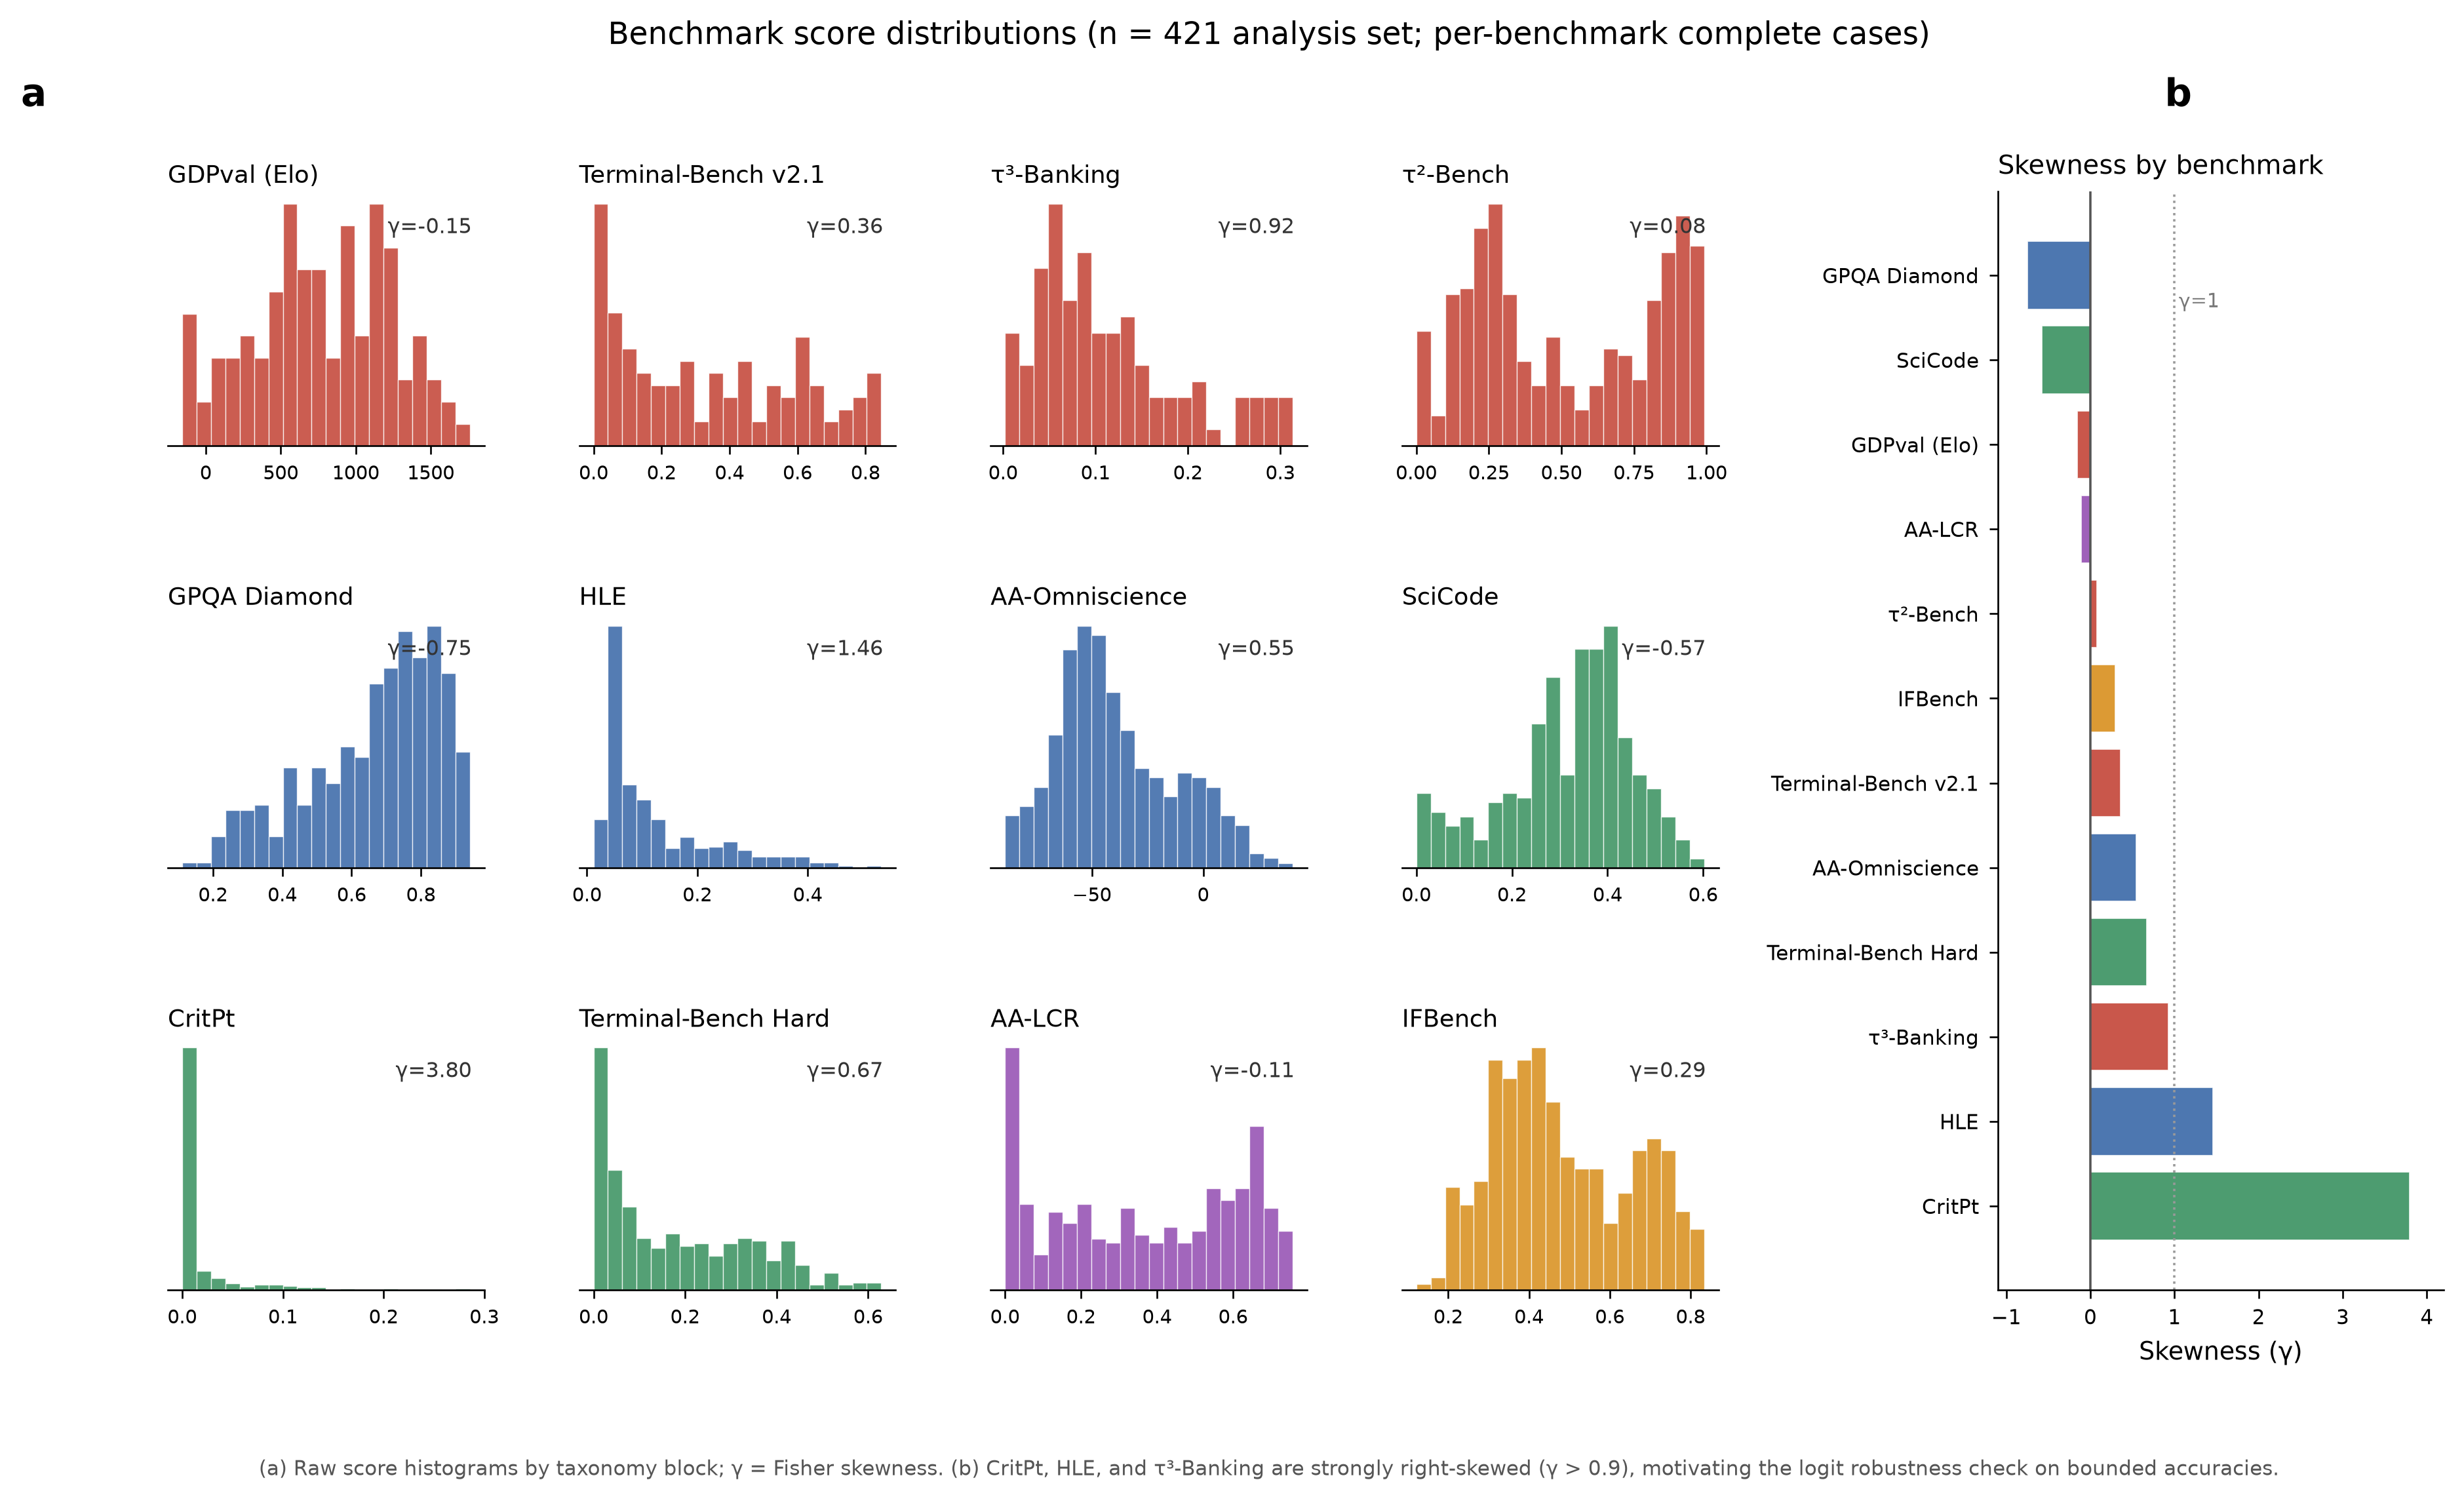
\includegraphics[width=\linewidth]{suppl_eda_distributions}
  \caption[Univariate score distributions and skewness]{\textbf{Univariate benchmark score
  distributions.} (a) Raw score histograms for the twelve benchmarks, coloured by capability block;
  $\gamma$ is the Fisher skewness. (b) Skewness ordered across benchmarks. Most benchmarks are bounded
  accuracies in $[0,1]$, and several are strongly right-skewed (CritPt $\gamma=3.8$, HLE $\gamma=1.5$,
  $\tau^3$-Banking $\gamma=0.9$), with scores concentrated near the floor. This boundedness motivates the
  logit-transform robustness check of Section~\ref{sec:robustness}. GDPval (Elo) and AA-Omniscience are
  on unbounded scales and are closer to symmetric.}
  \label{fig:eda_dist}
\end{figure}

\begin{figure}[htbp]
  \centering
  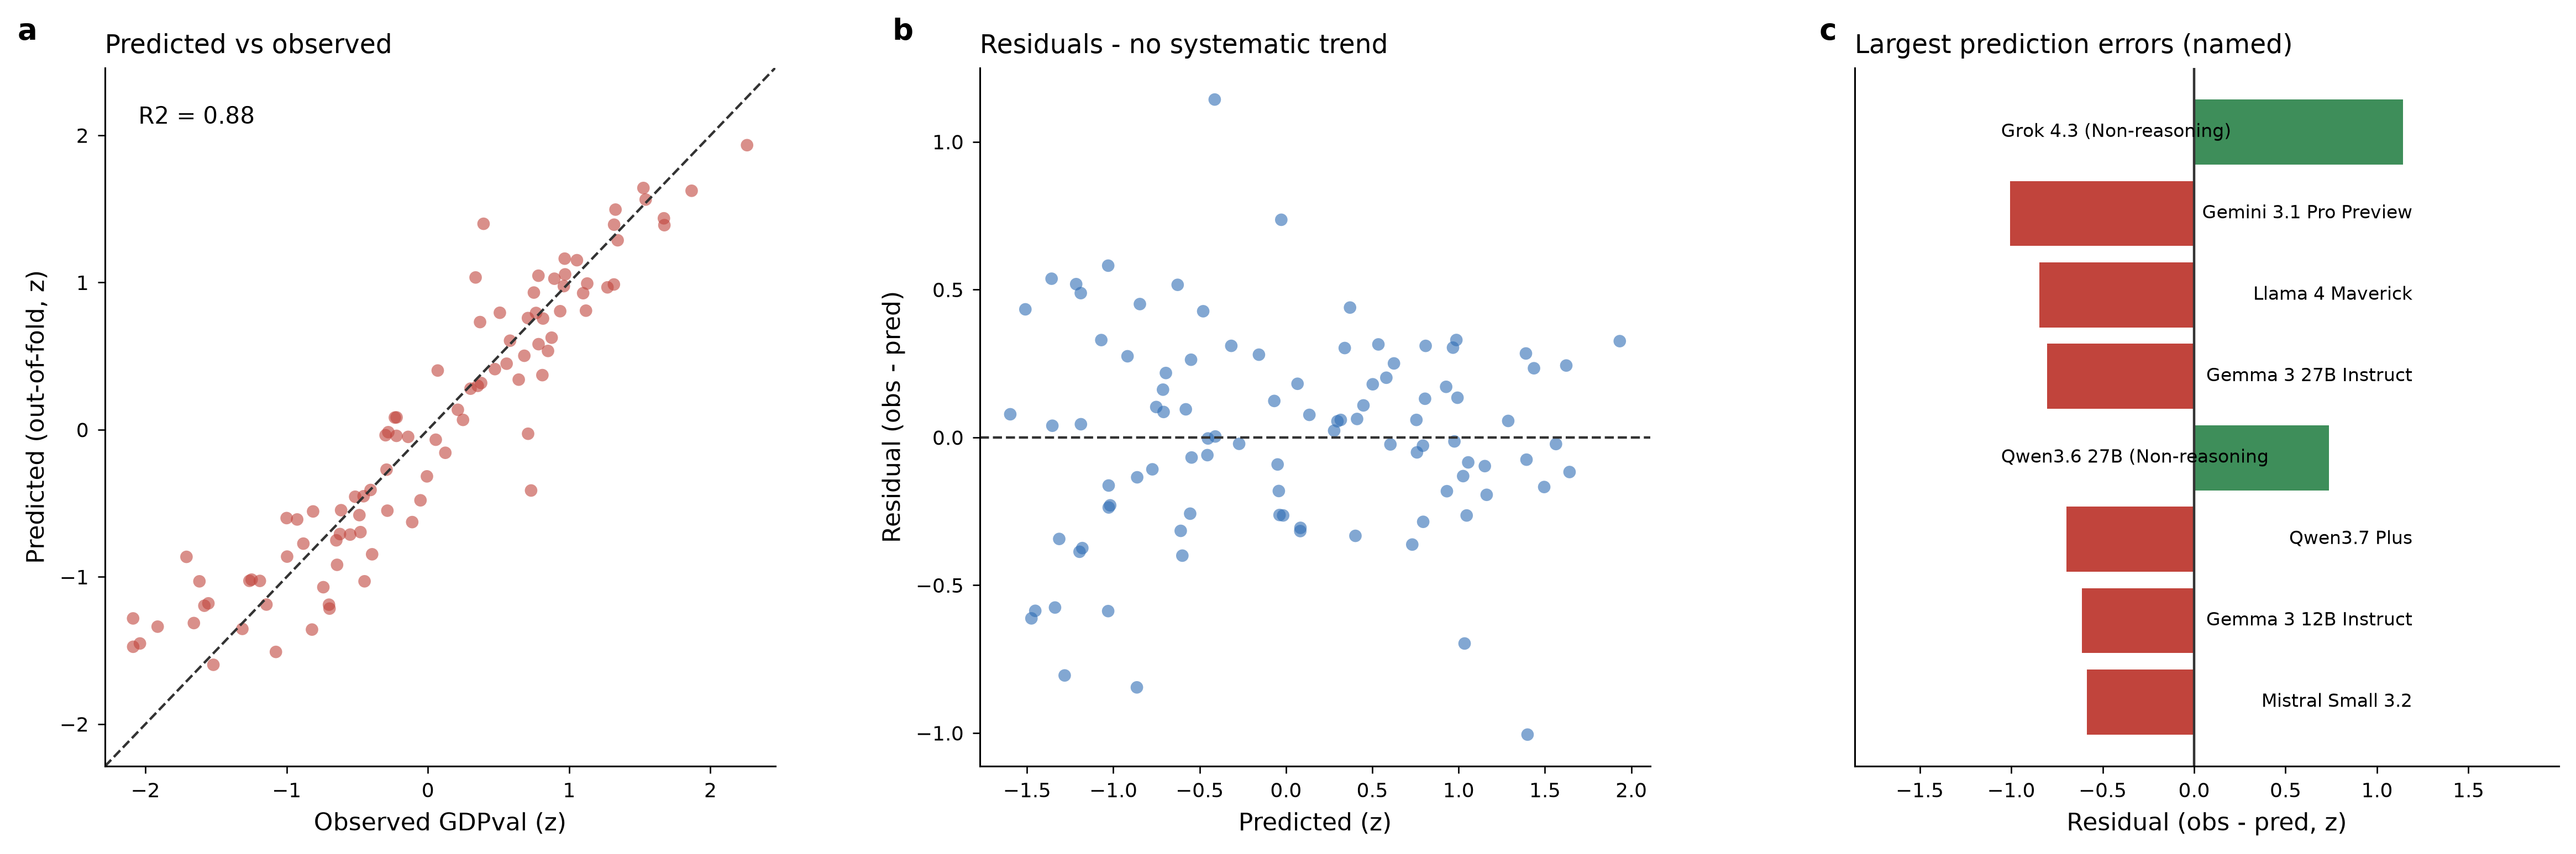
\includegraphics[width=\linewidth]{fig5_diagnostics}
  \caption[Regression diagnostics for the GDPval model]{\textbf{Regression diagnostics for the GDPval $k$-factor ridge model, out-of-fold.}
  (a) Predicted versus observed, on the identity line with $R^2=0.88$. (b) Residuals versus predicted
  show no systematic trend. (c) The eight largest residuals, named; these are interpretable outliers
  rather than evidence of misspecification.}
  \label{fig:diag}
\end{figure}

\begin{figure}[htbp]
  \centering
  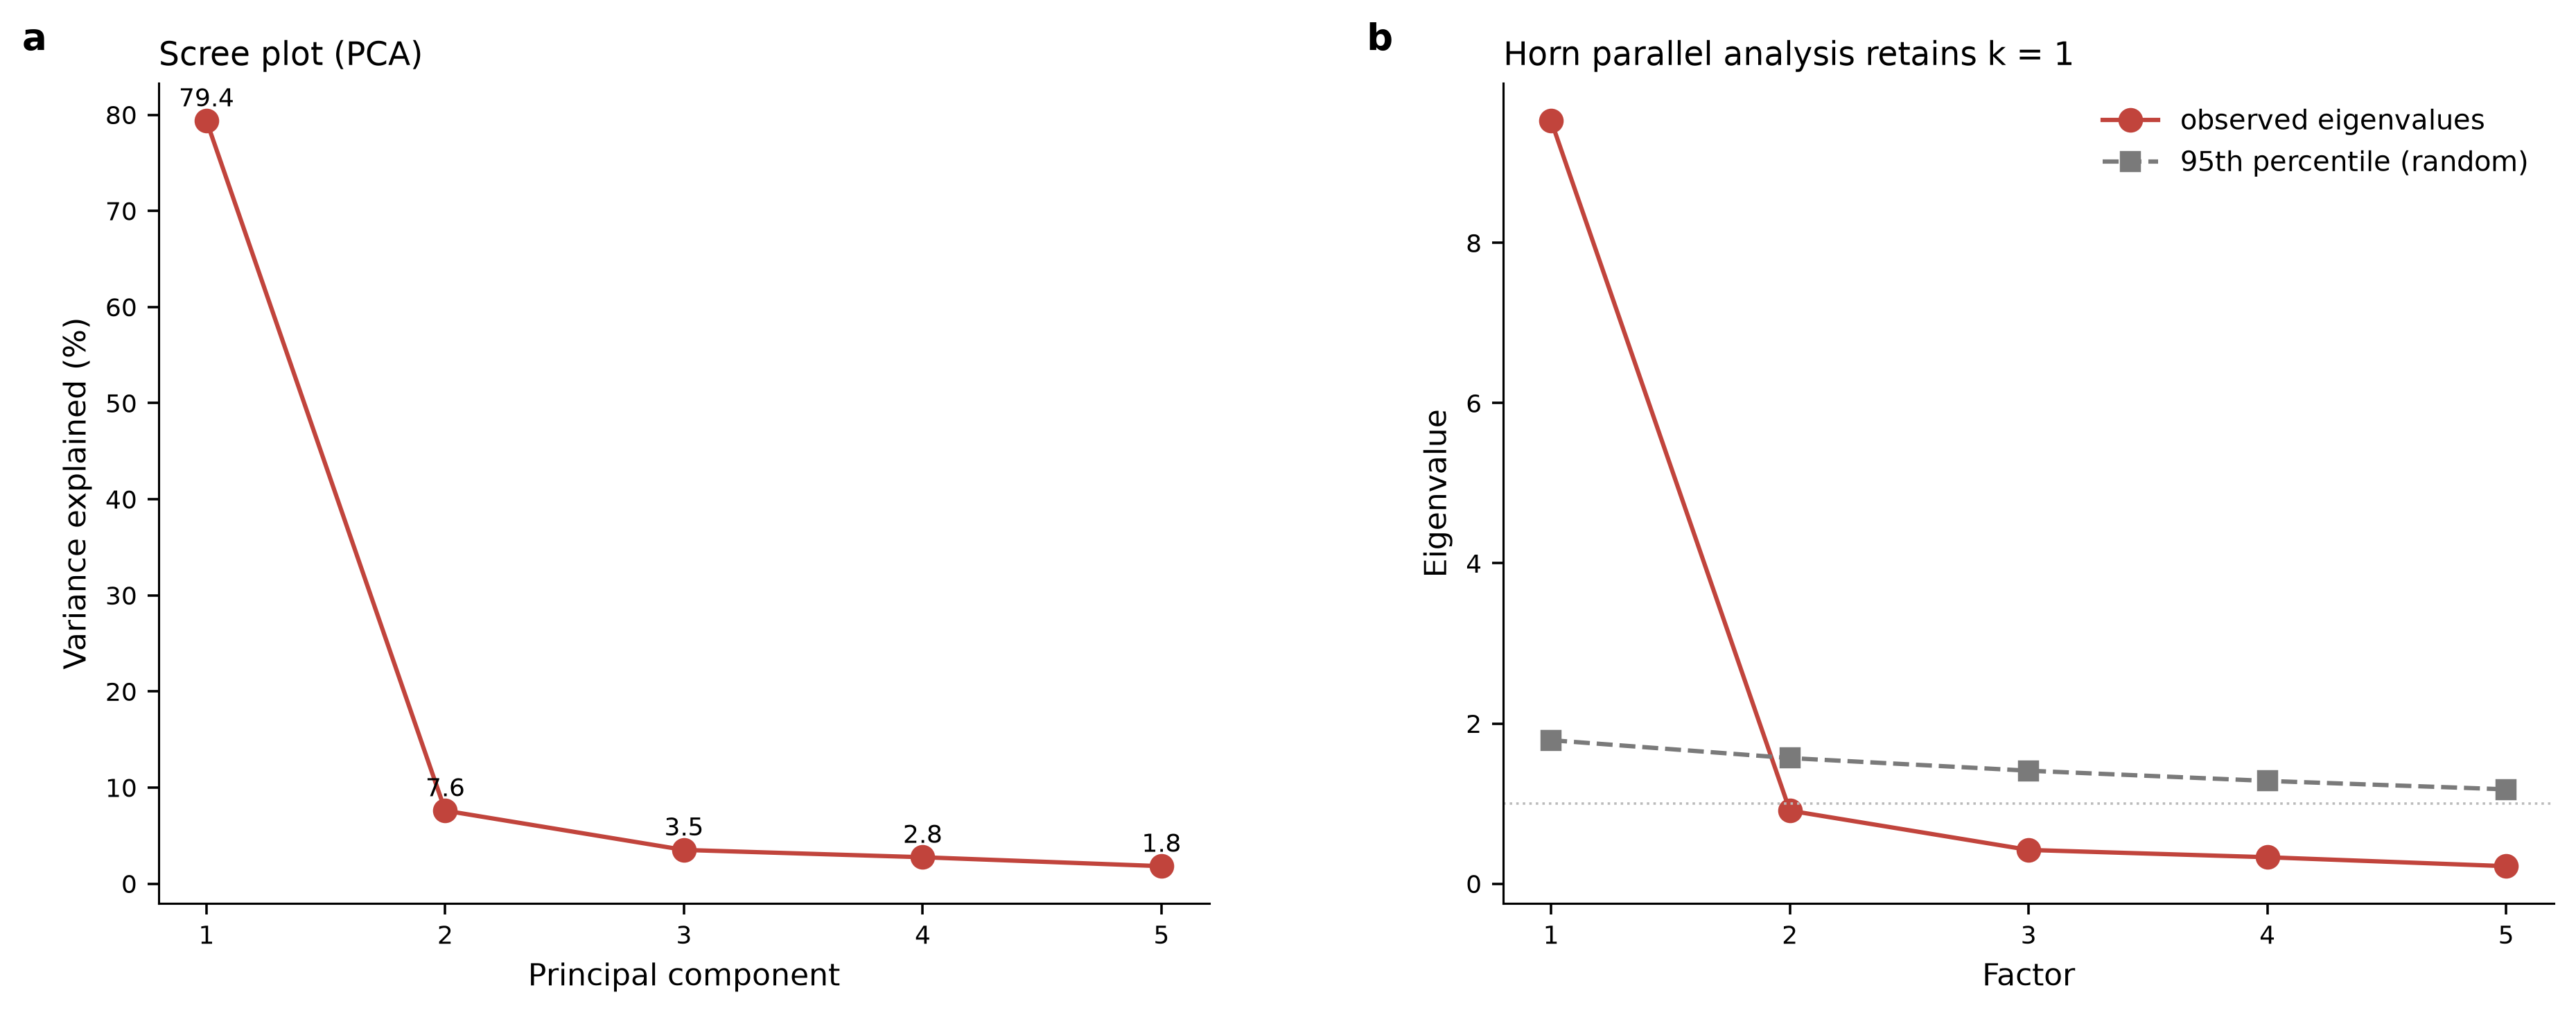
\includegraphics[width=\linewidth]{suppl_scree_parallel}
  \caption[Scree plot and Horn parallel analysis]{\textbf{Dimensionality of the battery.} (a) The scree plot of principal-component variance
  shares drops sharply after the first component (79.4\%). (b) Horn parallel analysis retains a single
  factor, since only the first observed eigenvalue (9.53) exceeds its random-data 95th percentile (1.79),
  while the second (0.91) already falls below (1.57). Values are computed in the notebook and stored in
  \texttt{parallel\_analysis.csv}.}
  \label{fig:scree}
\end{figure}

\begin{figure}[htbp]
  \centering
  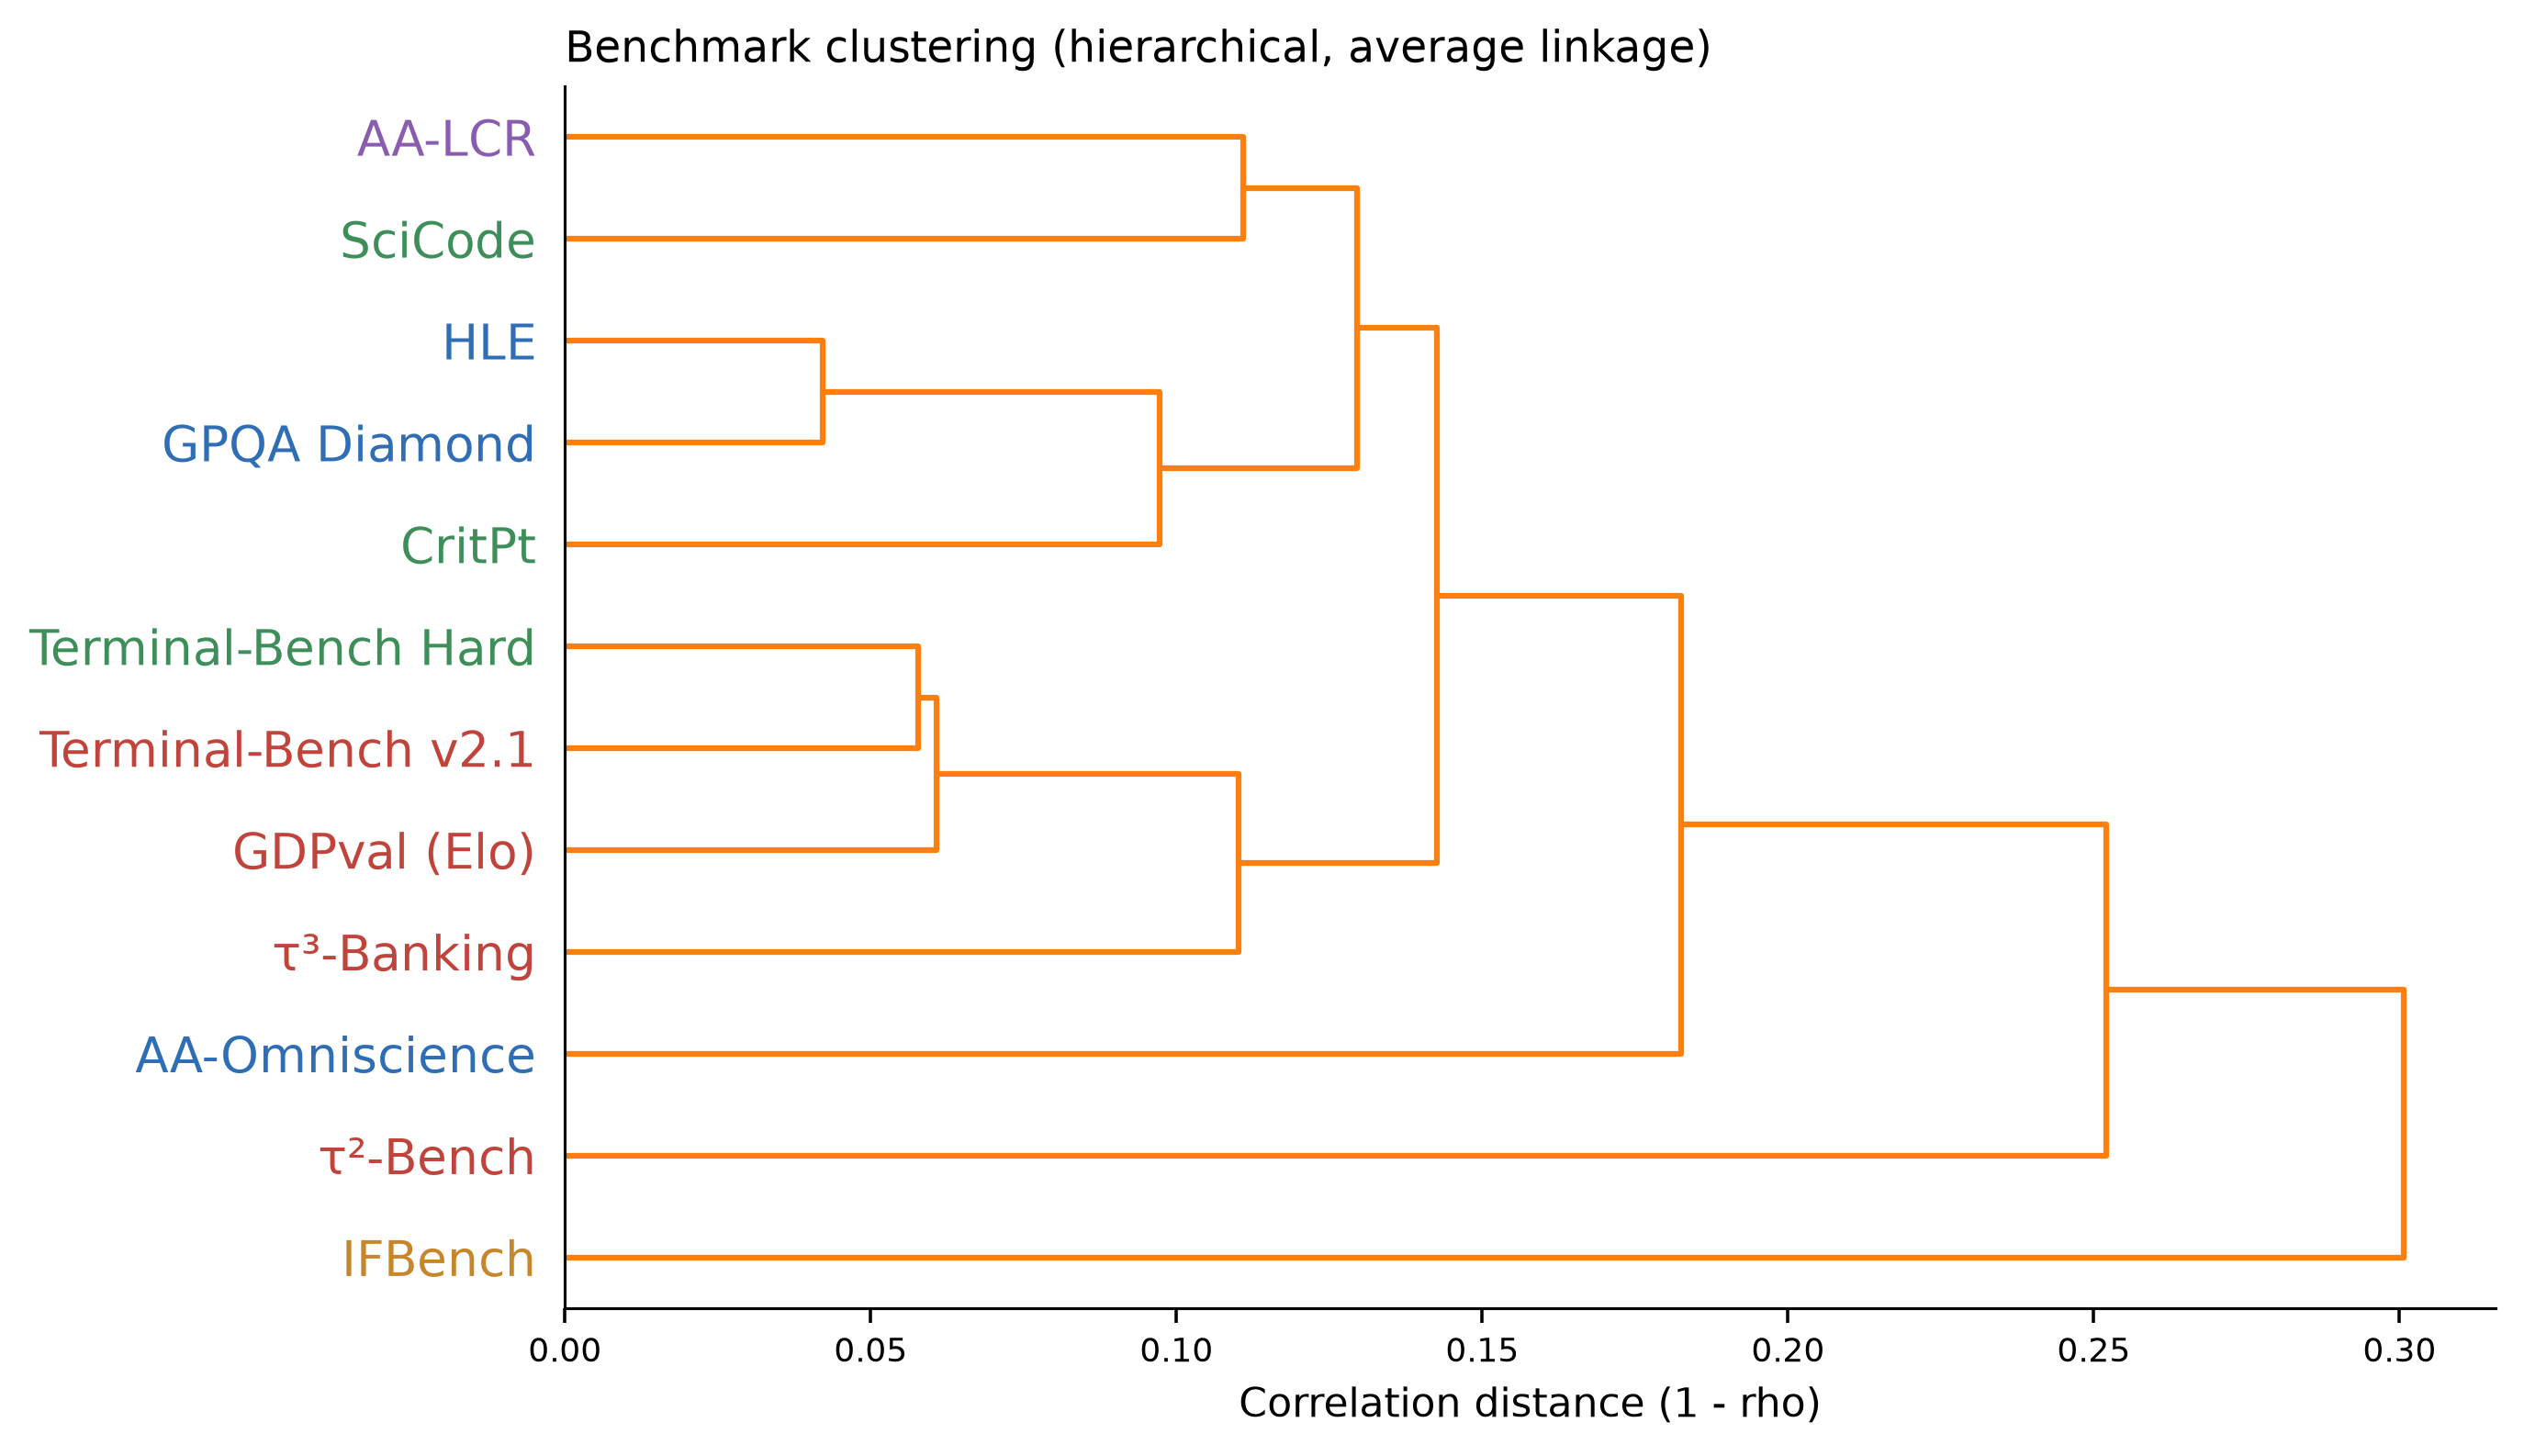
\includegraphics[width=\linewidth]{suppl_benchmark_dendrogram}
  \caption[Benchmark clustering dendrogram]{\textbf{Benchmark clustering by correlation distance} ($1-\rho$, average linkage). Ten of the
  twelve benchmarks, including three of four economic benchmarks, fall in one block, with $\tau^2$-Bench
  and IFBench branching separately.}
  \label{fig:dendro}
\end{figure}

\end{document}
